\documentclass[a4paper,20pt,oneside]{book}
\usepackage[utf8]{inputenc} 
\usepackage[T1]{fontenc} 
\usepackage[nonumberlist]{glossaries} 
\usepackage[english,ngerman]{babel}
\usepackage{float}
\usepackage{graphicx}
\usepackage{longtable}
\usepackage{titlesec}
\usepackage{pdfpages}
\usepackage{glossaries}
\usepackage{listings}
\usepackage{color}
\usepackage{titlepic}
\usepackage[DIV=14,BCOR=2mm,headinclude=true,footinclude=false]{typearea}
\definecolor{dkgreen}{rgb}{0,0.6,0}
\definecolor{gray}{rgb}{0.5,0.5,0.5}
\definecolor{mauve}{rgb}{0.58,0,0.82}
\lstset{frame=tb,
  language=bash,
  aboveskip=3mm,
  belowskip=3mm,
  showstringspaces=false,
  columns=flexible,
  basicstyle={\small\ttfamily},
  numbers=none,
  numberstyle=\tiny\color{gray},
  keywordstyle=\color{blue},
  commentstyle=\color{dkgreen},
  stringstyle=\color{mauve},
  breaklines=true,
  breakatwhitespace=true,
  tabsize=3
}
\titleformat{\subparagraph}
    {\normalfont\normalsize\bfseries}{\thesubparagraph}{1em}{}
\titlespacing*{\subparagraph}{\parindent}{3.25ex plus 1ex minus .2ex}{.75ex plus .1ex}

\makeglossaries

\newglossaryentry{Lambda-Entwickler}{
name = {Entwickler},
description = {ist ein User, der Lambdas durch die geeignete API-Schnittstelle hochlädt, verändert, löscht oder ausführt}}

\newglossaryentry{Lambda-Verwender}{
name = {Benutzer},
description = {ist ein User, der Lambdas aus ihrem entsprechenden \Gls{Docker}-\Gls{Container} mit Parameter aufruft}}

\newglossaryentry{Lambda-Funktion}{
name = {Lambda-Funktion},
plural = {Lambda-Funktionen},
description = {ist eine zustandslose Funktion}}

\newglossaryentry{Serverless}{
	name = {Serverless},
	description = {ist ein Konzept in der Softwaretechnik in dem Entwickler für das Managen und Provisionieren der Server nicht mehr selbst verantwortlich sein müssen}}

\newglossaryentry{Industrie 4.0}{
	name = {Industrie 4.0},
	description = { ist ein Begriff, der auf die Forschungsunion der deutschen Bundesregierung und ein gleichnamiges Projekt in der Hightech-Strategie der Bundesregierung zurückgeht, er bezeichnet ebenfalls eine Forschungsplattform. Die industrielle Produktion soll mit moderner Informations- und Kommunikationstechnik verzahnt werden. Technische Grundlage hierfür sind intelligente und digital vernetzte Systeme. Mit ihrer Hilfe soll eine weitestgehend selbst-organisierte Produktion möglich werden: Menschen, Maschinen, Anlagen, Logistik und Produkte kommunizieren und kooperieren in der Industrie 4.0 direkt miteinander. Durch die Vernetzung soll es möglich werden, nicht mehr nur einen Produktionsschritt, sondern eine ganze Wertschöpfungskette zu optimieren. Das Netz soll zudem alle Phasen des Lebenszyklus des Produktes einschließen – von der Idee eines Produkts über die Entwicklung, Fertigung, Nutzung und Wartung bis hin zum Recycling}}
	
\newglossaryentry{Rechenzeit}{
	name = {Rechenzeit (auch Laufzeit)},
	description = { ist die Zeit, die ein Programm bzw. eine \gls{Lambda-Funktion} zur Ausführung benötigt oder benötigt hat}}

\newglossaryentry{Softwareverteilung}{
	name = {Softwareverteilung (englisch software deployment)},
	description = {nennt man Prozesse zur Installation von Software auf Rechnern}}

\newglossaryentry{Skalierung}{
	name = {Skalierung (auch Skalierbarkeit)},
	description = {ist die Fähigkeit eines Systems aus Hard- und Software, die Leistung durch das Hinzufügen von Ressourcen – z. B. weiterer Hardware – in einem definierten Bereich proportional (bzw. linear) zu steigern}}

\newglossaryentry{Server}{
	name = {Server},
	description = {ist ein Computerprogramm oder ein Computer, der Computerfunktionalitäten wie Dienstprogramme, Daten oder andere Ressourcen bereitstellt, damit andere Computer oder Programme („Clients“) darauf zugreifen können, meist über ein Netzwerk}}
	
\newglossaryentry{REST}{
	name = {REST},
	description = { (Representional State Transfer) ist eine einfache Alternative zu anderen Verfahren zur Kommunikation zwischen Maschinen. Der größte Teil der von REST benötigten Infrastruktur ist bereits vorhanden, was die Verwendung sehr einfach macht}}
  
\newglossaryentry{skalierbar}{
	name = {skalierbar},
	description = {siehe Skalierung}}

\newglossaryentry{Konfiguration}{
	name = {Konfiguration},
	plural = {Konfigurationen},
	description = {ist eine Menge von Einstellungen, die eine \gls{Lambda-Funktion} zur Ausführung benötigt}}
	
\newglossaryentry{Token}{
	name = {Token},
	plural = {Tokens},
	description = {ist eine Komponente zur Identifizierung und Authentifizierung von Benutzern. In diesem Fall in Form von einer Textdatei.}}
	
\newglossaryentry{Repository}{
	name = {Repository},
	plural = {Repositorys},
	description = {ist ein verwaltetes (Online-) Verzeichnis zur Speicherung und Beschreibung von digitalen Objekten für ein digitales Archiv}}

\newglossaryentry{Serverbetreiber}{
	name = {Serverbetreiber},
	plural = {Serverbetreiber},
	description = { ist die Person, die die Software auf einem Server ausführen lässt und anderen Benutzern die Funktionalität der Software bereitstellt}}

\newglossaryentry{Internet of Things}{
	name = {Internet of Things},
	description = {ist die Zusammenarbeit von physischen Geräten, Fahrzeugen (auch als "connected devices" und "smart devices" bezeichnet), Gebäuden und anderen - ausgestattet mit Elektronik, Software, Sensoren, Motoren und Netzwerkverbindung, was es den Objekten ermöglicht, Daten zu sammeln und auszutauschen}}

\newglossaryentry{Webanwendung}{
	name = {Webanwendung},
	plural = {Webanwendungen},
	description = { ist ein Anwendungsprogramm, das beim Benutzer in einem Webbrowser abläuft bzw. dargestellt wird}}

\newglossaryentry{API}{
	name = {API},
	description = { ist ein Programmteil, der von einem Softwaresystem anderen Programmen zur Anbindung an das System zur Verfügung gestellt wird.}}
	
\newglossaryentry{App}{
	name = {App},
	plural = {Apps},
	description = { ist ein Computerprogramm, das eine für den Anwender nützliche \gls{Lambda-Funktion} ausführt}}
	
\newglossaryentry{zustandslos}{
	name = {zustandslos},
	description = {ist ein System oder Protokoll, welches keine Zustandsinformationen speichert}}
	
\newglossaryentry{gekapselt}{
	name = {gekapselt},
	description = {isoliert}}
	
\newglossaryentry{IntelliJ}{
	name = {IntelliJ},
	description = {ist eine Entwicklungsumgebung speziell für Java von der Firma JetBrains, die die wichtigsten Java-Technologien unterstützt}}
	
\newglossaryentry{Eclipse}{
	name = {Eclipse},
	description = {ist eine Entwicklungsumgebung der Firma Eclipse Foundation, die vor allem für Java-Entwicklung verwendet wird, aber auch viele andere Sprachen unterstützt}}
\newglossaryentry{Docker}{
	name = {Docker},
	description = {ist eine Open-Source-Software, die dazu verwendet werden kann, Anwendungen mithilfe von Betriebssystemvirtualisierung in \Gls{Container}n zu isolieren}}
\newglossaryentry{Container}{
	name = {Container},
	description = {ist ein lauffähiges, virtuelles Betriebssystem.}}
	
\newglossaryentry{python2}{
	name = {python2},
	description = {ist eine universelle, üblicherweise interpretierte höhere Programmiersprache.}}

\begin{document}
\titlepic{
\includegraphics[width=14cm]{Logo.png}}
\title{\Huge{\bfseries{Serverless Server for Industry 4.0}}}
\author{}
\date{November 2016}
\maketitle
\clearpage


\tableofcontents


\chapter{Einleitung}
Das Ziel dieses Projekt ist es, ein System zu schaffen, in dem  Entwickler einfach servergebundene Software implementieren können. Derzeit ist der Entwicklungsvorgang einer servergebundenen Software eng mit dem Konfigurieren und Verwalten eines Servers verbunden. Diese Tätigkeiten brauchen viel Zeit, Geld und Arbeitskraft. Ziel ist es, Code für fast jeden Service mit minimalem Administrationsaufwand auszuführen. Es muss nur der Code hochgeladen werden und das System übernimmt alles, was zum Ausführen und Skalieren erforderlich ist. 
\\
Es ist nicht nötig, den ganzen Server mit Aufwand aufzusetzen und zu warten, was natürlich die Kosten verringert. Vorteil des Systems ist, dass es den Entwicklern ermöglicht, nur mit Code-Schreiben beschäftigt zu sein. 
Somit wird Entwicklern, die eine Anwendung schreiben, aber wenig Wissen über die Verteilung und Serveradministration besitzen, mit dem System das Leben erleichtert. 
\\
Zustandlose Lambda-Funktionen, die als Code von den Entwicklern hochgeladen werden können ermöglichen es, viele verschiedene Aufgaben mithilfe des Systems zu lösen und nebeneinander auszuführen.
\\
Zudem ist es möglich, Berechtigungen zum Ausführen der Software zu delegieren, sodass die Einsatzgebiete nicht nur in Industriebereichen, sondern ebenfalls in Webanwendungen, Apps und Anwendungen des kommenden Internet of Things liegen können.
\\
Im Folgenden werden zwei Zielgruppen unterschieden: \gls{Lambda-Entwickler} und \gls{Lambda-Verwender}. Unter \gls{Lambda-Entwickler} ist die Gruppe der Menschen gemeint, die \Glspl{Lambda-Funktion} entwickeln und diese ausführen und ändern dürfen. Unter \gls{Lambda-Verwender} ist die Gruppe gemeint, welche nur Berechtigung besitzen die \Gls{Lambda-Funktion} auszuführen. Somit ist der \gls{Lambda-Entwickler} ein \gls{Lambda-Verwender} mit mehr Berechtigungen.


 
\chapter{Zielbestimmung}
\section{Musskriterien}
\subparagraph{Musskriterien funktionaler Art}
\begin{itemize}
\item \Gls{Lambda-Entwickler} soll \Gls{Lambda-Funktion} mithilfe einer einfachen \Gls{REST} \Gls{API} hochladen können.
\item \Gls{Lambda-Entwickler} soll \Gls{Lambda-Funktion} mithilfe einer einfachen \Gls{REST} \Gls{API} ausführen können.
\item \Gls{Lambda-Entwickler} soll \Gls{Lambda-Funktion} mithilfe einer einfachen \Gls{REST} \Gls{API} löschen können.
\item \Gls{Lambda-Entwickler} soll \Gls{Lambda-Funktion} mithilfe einer einfachen \Gls{REST} \Gls{API} ändern können.
\item \Gls{Lambda-Entwickler} soll \Gls{Lambda-Funktion} mithilfe einer einfachen \Gls{REST} \Gls{API} benennen können.
\item \Glspl{Konfiguration} (z.B. Signatur, Funktionsparameter, Ausführungsanzahl) der \gls{Lambda-Funktion} sollen spezifiziert werden können.
\item \Gls{Lambda-Entwickler} sollen mithilfe eines \Glspl{Token} authentifiziert werden können.
\item \Gls{Lambda-Verwender} sollen mithilfe eines \Glspl{Token}, der vom \Gls{Lambda-Entwickler} ausgegeben wird authentifiziert werden können und mit diesem \gls{Token} \Glspl{Lambda-Funktion} ausführen.
\item Laufende Instanzen gelöschter \Glspl{Lambda-Funktion} sollen gestoppt werden.
\item \Glspl{Lambda-Funktion} sollen \Gls{zustandslos} sein.
\item \Glspl{Lambda-Funktion} sollen \Gls{gekapselt} werden.
\item \Glspl{Lambda-Funktion} dürfen nur eine vom \Gls{Server} spezifizierte Zeit lang laufen.
\end{itemize}
\subparagraph{Musskriterien nichtfunktionaler Art}
\begin{itemize}
\item Das System soll in Rechner- und Speicherressourcen  \gls{skalierbar} sein.
\item Das System soll als Mindestgrundlage \glspl{Lambda-Funktion} in python2 unterstützen.
\end{itemize}
\pagebreak
\section{Wunschkriterien}
\subparagraph{Wunschkriterien funktionaler Art}
\begin{itemize}
\item \Glspl{Lambda-Funktion} dürfen nur eine vom \Gls{Lambda-Verwender} spezifizierte Zeit lang laufen, sofern diese die maximale Laufzeit nicht übersteigt.
\item Zu jedem \Gls{Token} wird ein Zähler erstellt, der für statistische Zwecke ausgelesen werden kann.
\item \Gls{Lambda-Entwickler} können ein \Gls{Repository} angeben und von dort die \gls{Lambda-Funktion} auf den \Gls{Server} laden.
\item Versionsverwaltung der \Glspl{Lambda-Funktion}.
\item Der \Gls{Server} kann Firewall-Einstellungen für \Glspl{Lambda-Funktion} definieren.
\item \Gls{Lambda-Entwickler} können Firewall-Einstellungen für \Glspl{Lambda-Funktion} definieren, sofern sie nicht den \Gls{Server}-Einstellungen widersprechen.
\item Sofern die Ausführungszeit einer \Gls{Lambda-Funktion} ein Limit überschreitet, wird die HTTP-Verbindung abgebrochen und bei Beendigung der \Gls{Lambda-Funktion} wird das Ergebnis bereitgestellt.
\item Prepaid-Bezahlsystem für \Glspl{Token} abhängig von der Ausführungszeit der zugehörigen \Gls{Lambda-Funktion}.
\item Erwartete Laufzeit einer  \Gls{Lambda-Funktion} bereitstellen.
\end{itemize}

\subparagraph{Wunschkriterien nichtfunktionaler Art}
\begin{itemize}
\item Die Ausführung einer stark ressourcenaufwändigen \Gls{Lambda-Funktion} beeinträchtigt nicht die Ausführung anderer \Glspl{Lambda-Funktion} auf dem \Gls{Server}.
\item Das System soll um Sprachen für \Glspl{Lambda-Funktion} erweiterbar sein.
\end{itemize}

\section{Abgrenzungskriterien}
\begin{itemize}
\item Entwicklung einer graphischen Nutzeroberfläche.
\item Entwicklung einer Nutzerverwaltung mit Datenbank.
\end{itemize}


\chapter{Produkteinsatz}
Das System erleichtert das Leben der Softwareentwickler. Es übernimmt für diese Administrationsarbeiten wie \Gls{Server}wartung, \Gls{Softwareverteilung} und \Gls{Skalierung}. Damit ist das Hauptziel, den Entwicklungsvorgang einer Software zu beschleunigen und zu verfeinern. 
Zudem ist das System komfortabel für \Gls{Serverbetreiber}, welche mit wenig Aufwand das System aufsetzen und den unterliegenden Server Warten können.
\section{Anwendungsbereich} 
Das System soll für die Anwendung im Softwareentwicklungsbereich konstruiert werden. Das System wird für folgende Teilbereiche entworfen:
\begin{itemize}
	\item \Gls{Industrie 4.0}
	\item \Gls{Internet of Things}
	\item \Glspl{Webanwendung}
	\item \Glspl{App}
\end{itemize}
\section{Zielgruppen}
\begin{itemize} 
	\item Softwareentwickler
\end{itemize}
\section{Betriebsbedingungen}
\begin{itemize}
	\item Rechner
	\item Internetverbindung 
\end{itemize}

\chapter{Produktumgebung}
\section{Software}
Die folgende Software muss auf dem \Gls{Server} ausgeführt werden können:
\begin{itemize}
\item \Gls{Docker} als Laufzeitumgebung
\item Compiler/Interpreter für die unterstützen Sprachen
\end{itemize}
Das Betriebssystem des Servers muss diese Software ausführen können. Also bieten sich vor allem Windows, Linux oder Mac OS X als Betriebssystem des Servers an.

\section{Hardware}
Der Server muss genug Ressourcen haben, damit dort \Gls{Docker} lauffähig ist. Ausßerdem müssen dort viele \Glspl{Lambda-Funktion} gleichzeitig ausgeführt werden können.

\chapter{Funktionale Anforderungen}

\section{Überblick: Grundfunktionen}
\begin{longtable}{lp{10cm}l}
\hline \\
\textbf{Nr.} &  \textbf{Beschreibung} \\ \hline \hline \\ \endhead
 /F010/ & \glspl{Lambda-Funktion} hochladen\\ \hline \\ 
 /F011/ & Zugriffs-\gls{Token} zurückgeben \\ \hline \\
 /F020/ & \glspl{Lambda-Funktion} ausführen\\ \hline \\
 /F021/ & Ausführungsumgebung für \glspl{Lambda-Funktion} bereitstellen \\ \hline \\
 /F030/& \glspl{Lambda-Funktion} löschen\\ \hline \\
 /F031/ & Beendigung von Instanzen gelöschter \glspl{Lambda-Funktion} \\ \hline \\
 /F040/& \glspl{Lambda-Funktion} updaten \\ \hline \\
 /F050/& \glspl{Lambda-Funktion} benennen \\ \hline \\
 /F060/& \glspl{Lambda-Funktion} konfigurieren \\ \hline \\
 /F080/& Zeitabhängige Terminierung von \glspl{Lambda-Funktion} \\ \hline \\
 /F090/& Daten für \gls{Lambda-Funktion} einbinden \\ \hline \\
 /F100/& \gls{Lambda-Entwickler} authentifizieren\\ \hline \\
 /F110/& \gls{Lambda-Entwickler} soll \glspl{Token} zur Ausführung einer \gls{Lambda-Funktion} erzeugen können\\ \\
\hline 
\hline
\end{longtable}
\pagebreak

\section{Überblick: Erweiterte Funktionen}
\begin{longtable}{lp{10cm}l}
\hline \\
\textbf{Nr.} &  \textbf{Beschreibung} \\ \hline\hline \\ \endhead
 /F140/& \gls{Lambda-Entwickler} sollen eine maximale Laufzeit spezifizieren können, die nicht die vom Server vorgegebene maximale Laufzeit überschreitet\\ \hline \\
 /F150/& Zähler zu \glspl{Token} speichern\\ \hline \\
 /F160/& Zähler zu \glspl{Token} auslesen\\ \hline \\
 /F170/& \gls{Lambda-Entwickler} sollen \glspl{Repository} zum Hochladen von \glspl{Lambda-Funktion} spezifizieren können \\ \hline \\
 /F180/& Versionsverwaltung für hochgeladene \glspl{Lambda-Funktion}\\ \hline \\
 /F190/& \gls{Lambda-Entwickler} soll Firewalleinstellung für \glspl{Lambda-Funktion} spezifizieren können \\ \hline \\
/F200/& spätere Bereitstellung des Ergebnisses für \glspl{Lambda-Funktion}\\ \hline \\
/F210/& \gls{Lambda-Entwickler} soll \glspl{Token} kaufen können (Prepaid)\\ \hline \\
/F220/& \gls{Serverbetreiber} kann Statistiken einsehen\\ \\
\hline
\hline
\end{longtable}
\hspace{3cm}
\section{Detaillierte Beschreibung}
\subsection{Grundfunktionen}
\subparagraph{/F010/}
\textbf{Kurzbeschreibung:} Hochladen einer \Gls{Lambda-Funktion}
\\
\textbf{Vorbedingung:} \Gls{Lambda-Entwickler} besitzt eine \gls{Lambda-Funktion}
\\
\textbf{Beschreibung:} Ein \Gls{Lambda-Entwickler} schickt eine Upload-Anfrage an den \Gls{Server} über die spezifizierte \gls{REST} \Gls{API}. Dort wird auf mögliche Fehler geprüft, dann wird die neue \Gls{Lambda-Funktion} hinzugefügt, falls kein Fehler aufgetreten ist. /F021/ wird ausgeführt. /F011/ wird ausgeführt.
\\
\textbf{Nachbedingung:} Die \Gls{Lambda-Funktion} ist auf dem \Gls{Server} vorhanden und kann verwendet werden.

\subparagraph{/F011/}
\textbf{Kurzbeschreibung:} Rückgabe eines \Glspl{Token} zum Zugriff auf eine \Gls{Lambda-Funktion}
\\
\textbf{Vorbedingung:} Die \Gls{Lambda-Funktion} ist auf dem \Gls{Server} vorhanden.
\\
\textbf{Beschreibung:} Der \Gls{Server} gibt einen \Gls{Token} an den \Gls{Lambda-Entwickler} zurück, mit dem er auf die \Gls{Lambda-Funktion} zugreifen kann.
\\
\textbf{Nachbedingung:} Der \Gls{Token} kann zum Zugriff auf die \Gls{Lambda-Funktion} verwendet werden.

\subparagraph{/F020/}
\textbf{Kurzbeschreibung:} Ausführung einer \Gls{Lambda-Funktion}
\\
\textbf{Vorbedingung:} Die \Gls{Lambda-Funktion} ist auf dem \Gls{Server} vorhanden und der \Gls{Lambda-Verwender} hat den benötigten \Gls{Token}. Dies ist entweder der \Gls{Token} des Entwicklers oder ein vom Entwickler für \Gls{Lambda-Verwender} erzeugter \Gls{Token} (siehe /F110/).
\\
\textbf{Beschreibung:} Der \Gls{Server} startet die Ausführung einer \Gls{Lambda-Funktion} und übergibt ihr die vom \Gls{Lambda-Verwender} übergebenen Daten. Nach der Ausführung liegt ein Ergebnis vor, das wieder an den \gls{Lambda-Verwender} zurückgegeben wird.
\\
\textbf{Nachbedingung:} Der \Gls{Server} hat danach den gleichen Zustand wie vor der Ausführung. 

\subparagraph{/F021/}
\textbf{Kurzbeschreibung:} Bereitstellung einer Umgebung in der eine \Gls{Lambda-Funktion} ausgeführt werden kann.
\\
\textbf{Vorbedingung:} Die \Gls{Lambda-Funktion} ist auf dem \Gls{Server} vorhanden.
\\
\textbf{Beschreibung:} Der \Gls{Server} erstellt eine Ausführungsumgebung für eine \Gls{Lambda-Funktion}, die z.B. Bibliotheken, die zur Ausführung benötigt werden, Software oder Daten beinhaltet. Außerdem werden so die Ausführungen \gls{gekapselt}. 
\\
\textbf{Nachbedingung:} Die Ausführungsumgebung wird gelöscht, wenn sie nicht mehr benötigt wird.

\subparagraph{/F030/}
\textbf{Kurzbeschreibung:} Löschen einer \Gls{Lambda-Funktion}
\\
\textbf{Vorbedingung:} Die \Gls{Lambda-Funktion} ist auf dem \Gls{Server} vorhanden und der \Gls{Lambda-Entwickler} hat den benötigten \Gls{Token} zur Authorisierung.
\\
\textbf{Beschreibung:} Ein \Gls{Lambda-Entwickler} benutzt seinen \Gls{Token} um eine \Gls{Lambda-Funktion} vom \Gls{Server} zu entfernen. /F031/ wird ausgeführt.
\\
\textbf{Nachbedingung:} Die \Gls{Lambda-Funktion} ist nicht mehr auf dem \Gls{Server} vorhanden und laufende Instanzen werden beendet.

\subparagraph{/F031/}
\textbf{Kurzbeschreibung:} Beendigung aller laufender Instanzen einer gelöschten \Gls{Lambda-Funktion}
\\
\textbf{Vorbedingung:} Die \Gls{Lambda-Funktion} wurde gelöscht.
\\
\textbf{Beschreibung:} Der \Gls{Server} beendet alle laufenden Instanzen einer \Gls{Lambda-Funktion} die von ihrem Entwickler gelöscht wurde.
\\
\textbf{Nachbedingung:} Auf dem \Gls{Server} laufen keine Instanzen der gelöschten \Gls{Lambda-Funktion} mehr.

\subparagraph{/F040/}
\textbf{Kurzbeschreibung:} Ändern einer bereits vorhandenen \Gls{Lambda-Funktion}
\\
\textbf{Vorbedingung:} Die \Gls{Lambda-Funktion} ist auf dem \Gls{Server} vorhanden und der \Gls{Lambda-Entwickler} hat den benötigten \Gls{Token} zur Authorisierung.
\\
\textbf{Beschreibung:} Ein \Gls{Lambda-Entwickler} benutzt seinen \Gls{Token} um eine auf dem \Gls{Server} vorhandene \Gls{Lambda-Funktion} zu ändern (z.B. zur Fehlerkorrektur oder zur Erweiterung).
\\
\textbf{Nachbedingung:} Die neue Version der \Gls{Lambda-Funktion} ist auf dem \Gls{Server} vorhanden.

\pagebreak

\subparagraph{/F050/}
\textbf{Kurzbeschreibung:} Benennen einer \Gls{Lambda-Funktion}
\\
\textbf{Vorbedingung:} \Gls{Lambda-Entwickler} besitzt gewünschte Benennung einer \Gls{Lambda-Funktion}.
\\
\textbf{Beschreibung:}
Fall 1: \Gls{Lambda-Funktion} noch nicht auf dem \gls{Server} vorhanden.\\
Ein \Gls{Lambda-Entwickler} spezifiziert in der Konfiguration der \Gls{Lambda-Funktion} die Benennung der \gls{Lambda-Funktion}\\
Fall 2: \Gls{Lambda-Funktion} auf dem \gls{Server} vorhanden.\\
Ein \Gls{Lambda-Entwickler} benutzt seinen \Gls{Token} um eine auf dem \Gls{Server} vorhandene \Gls{Lambda-Funktion} zu benennen. (siehe /F040/)
\\
\textbf{Nachbedingung:} Die \Gls{Lambda-Funktion} kann in Zukunft über den vergebenen Namen angesprochen werden.

\subparagraph{/F060/}
\textbf{Kurzbeschreibung:} Konfigurieren einer \Gls{Lambda-Funktion}
\\
\textbf{Vorbedingung:} Die \Gls{Lambda-Funktion} ist auf dem \Gls{Server} vorhanden und der \Gls{Lambda-Verwender} hat den benötigten \Gls{Token} zur Authorisierung.
\\
\textbf{Beschreibung:} Ein \Gls{Lambda-Verwender} benutzt seinen \Gls{Token} um für eine auf dem \Gls{Server} vorhandene \Gls{Lambda-Funktion} eine \Gls{Konfiguration} zur Ausführung festzulegen. /F020/ wird ausgeführt.
\\
\textbf{Nachbedingung:} Ausführungs-Instanzen der \Gls{Lambda-Funktion} verwenden die andere Konfigurationen.

\subparagraph{/F080/}
\textbf{Kurzbeschreibung:} Zeitabhängiges Beenden einer \Gls{Lambda-Funktion}
\\
\textbf{Vorbedingung:} Auf dem \Gls{Server} ist eine Maximallaufzeit definiert.
\\
\textbf{Beschreibung:} Der \Gls{Server} beendet jede \Gls{Lambda-Funktion}, deren Ausführung die Maximallaufzeit überschreitet, damit der \Gls{Server} nicht von zu lange laufenden Instanzen der \glspl{Lambda-Funktion} blockiert wird. 
\\
\textbf{Nachbedingung:} Die laufende Instanz von der \Gls{Lambda-Funktion} wird nach Überschreitung der Maximallaufzeit terminiert.

\subparagraph{/F090/}
\textbf{Kurzbeschreibung:} Einbindung von Daten für eine \Gls{Lambda-Funktion}
\\
\textbf{Vorbedingung:} Die \Gls{Lambda-Funktion} ist auf dem \Gls{Server} vorhanden und der \Gls{Lambda-Verwender} hat den benötigten \Gls{Token} zur Authorisierung.
\\
\textbf{Beschreibung:} Ein \Gls{Lambda-Verwender} verwendet einen \Gls{Token} um festzulegen, mit welchen Daten eine \Gls{Lambda-Funktion} ausgeführt werden soll. Der \Gls{Server} holt diese Daten und bindet sie in die Ausführungsumgebung ein (siehe /F021/).
\\
\textbf{Nachbedingung:} Die \Gls{Lambda-Funktion} kann mit den angegebenen Daten ausgeführt werden.

\subparagraph{/F100/}
\textbf{Kurzbeschreibung:} Authentifizierung der \Glspl{Lambda-Entwickler}
\\
\textbf{Vorbedingung:} Die \Gls{Lambda-Funktion} ist auf dem \Gls{Server} vorhanden und der \Gls{Lambda-Entwickler} hat den benötigten \Gls{Token} zur Authorisierung.
\\
\textbf{Beschreibung:} Ein \Gls{Lambda-Entwickler} authentifiziert sich mit einem vorher erworbenen \Gls{Token} beim \Gls{Server}.
\\
\textbf{Nachbedingung:} Dem \Gls{Lambda-Entwickler} ist es nun möglich Operationen auf \Glspl{Lambda-Funktion} durchzuführen (z.B. ändern, löschen).

\pagebreak

\subparagraph{/F110/}
\textbf{Kurzbeschreibung:} Erzeugung von \Glspl{Token} zur Ausführung einer \Gls{Lambda-Funktion}
\\
\textbf{Vorbedingung:} Die \Gls{Lambda-Funktion} ist auf dem \Gls{Server} vorhanden.
\\
\textbf{Beschreibung:} Ein \Gls{Lambda-Entwickler} erzeugt \Glspl{Token} für \Gls{Lambda-Verwender}, mit denen diese die Berechtigung haben eine bestimmte \Gls{Lambda-Funktion} auszuführen.
\\
\textbf{Nachbedingung:} Die \Gls{Lambda-Funktion} kann mit den erzeugten \Glspl{Token} ausgeführt werden.
\\
\subsection{Erweiterte Funktionen}
\iffalse
\subparagraph{/F140/}
\textbf{Kurzbeschreibung:} \gls{Lambda-Entwickler} soll eine Laufzeit spezifizieren können, die nicht die maximale Laufzeit überschreitet
\\
\textbf{Vorbedingung:} \gls{Lambda-Entwickler} muss sich über bestimmte Laufzeit einer \gls{Lambda-Funktion} entscheiden.
\\
\textbf{Beschreibung:} \gls{Lambda-Entwickler} hat eine Möglichkeit, eine Laufzeitgrenze einer \gls{Lambda-Funktion} festlegen, d.h. wenn z.B. \gls{Lambda-Entwickler} für \gls{Lambda-Funktion} F die Laufzeitgrenze 5 Sekunden gesetzt hat, dann kann diese \gls{Lambda-Funktion} F nicht länger als in Zeitraum von 5 Sekunden ausgeführt sein werden. Diese Laufzeitgrenze kann nicht die Maximale Laufzeit unseres Systems (d.h. die maximale Zeit, die von unserem System definiert ist) überschreiten.
\\
\textbf{Nachbedingung:} Eine \gls{Lambda-Funktion} darf nicht mehr als vorspezifizierte Zeit laufen.
\subparagraph{/F150/}
\textbf{Kurzbeschreibung:} Zähler zu \gls{Token} erstellen.
\\
\textbf{Vorbedingung:} ein \gls{Token} zur Verfügung, der beim Hochladen einer \gls{Lambda-Funktion} zurückgegeben war. 
\\
\textbf{Beschreibung:} man erstellt einen Zähler für \gls{Token}. Nachdem eine \gls{Lambda-Funktion} ausgeführt wird, bekommt der Zähler die Information über wie viele Sekunden diese Ausführung gedauert hat.
\\
\textbf{Nachbedingung:} Zähler enthält Zeitinformation von letzter Ausführung einer \gls{Lambda-Funktion}.
\subparagraph{/F160/}
\textbf{Kurzbeschreibung:} Zähler zu \gls{Token} auslesen. 
\\
\textbf{Vorbedingung:} Existenz von einem Zähler zu einem \gls{Token}.
\\
\textbf{Beschreibung:} diese \gls{Lambda-Funktion} gibt die Zeit in Sekunden zurück, die der Zähler enthält. 
\\
\textbf{Nachbedingung:} Man hat die Zeit letzter Ausführungszeit zur Verfügung.
\subparagraph{/F170/}
\textbf{Kurzbeschreibung:} \gls{Lambda-Entwickler} soll repository zum \Glspl{Lambda-Funktion} hochladen spezifizieren können.
\\
\textbf{Vorbedingung:} Repository mit Dateien zur Verfügung, die Code von \Glspl{Lambda-Funktion} enthalten.
\\
\textbf{Beschreibung:} Wenn ein Nutzer schon die Dateien mit Code von \Glspl{Lambda-Funktion} in einem Repository hat, dann kann Nutzer einfach Repository spezifizieren. Dannach bekommt Nutzer eine Möglichkeit, die \Glspl{Lambda-Funktion} gerade aus vorspezifizierten Repository hochzuladen. 
\\
\textbf{Nachbedingung:} spezifiziertes Repository, woraus \Glspl{Lambda-Funktion} hochgeladen werden können.
\subparagraph{/F180/}
\textbf{Kurzbeschreibung:} Versionsverwaltung für hochgeladene. \glspl{Lambda-Funktion}
\\
\textbf{Vorbedingung:} Vorspezifiziertes Repository mit Lambda-Funktionen.
\\
\textbf{Beschreibung:} Man kann \Glspl{Lambda-Funktion} ändern. Alle Änderungen können mit verschidenen Versionen bezeichnet werden.
\\
\textbf{Nachbedingung:} \Glspl{Lambda-Funktion} können verschidene Versionen haben.
\subparagraph{/F190/}
\textbf{Kurzbeschreibung:} \gls{Lambda-Entwickler} soll Firewalleinstellung für \gls{Lambda-Funktion} spezifizieren können.
\\
\textbf{Vorbedingung:} Existierende \gls{Lambda-Funktion}.
\\
\textbf{Beschreibung:} Man kann sich entscheiden was eine \gls{Lambda-Funktion} machen darf und nicht darf. Z.B. man kann einen Datenbereich festlegen, zu dem die \gls{Lambda-Funktion} kein Zugriffsrecht hat.
\\
\textbf{Nachbedingung:} Begrenzte Zugriffsmöglichkeiten einer \gls{Lambda-Funktion}.

\subparagraph{/F200/}
\textbf{Kurzbeschreibung:} spätere Bereitstellung von einem Ergebnisses für \glspl{Lambda-Funktion}.
\\
\textbf{Vorbedingung:} ein Ergebniss, das eine \gls{Lambda-Funktion} zurückgegeben hat.
\\
\textbf{Beschreibung:} wenn man eine \gls{Lambda-Funktion} ausgeführt hat, kann man das Ergebniss dieser Ausführung speichern und für weitere Ziele benutzen. 
\\
\textbf{Nachbedingung:} Ergebniss nach der Ausführung einer \gls{Lambda-Funktion}.
\subparagraph{/F210/}
\textbf{Kurzbeschreibung:} \gls{Lambda-Entwickler} soll \gls{Token}s kaufen können (Prepaid).
\\
\textbf{Vorbedingung:} Geld.
\\
\textbf{Beschreibung:} Möglichkeit \gls{Token}s zu kaufen. Wenn man eine \gls{Lambda-Funktion} in unserem System ausführen will, dann muss man zuerst ein \gls{Token} für die \gls{Lambda-Funktion} kaufen. Dannach kann man die \gls{Lambda-Funktion} ausführen. 
\\
\textbf{Nachbedingung:} gekaufte \gls{Token} und Möglichkeit eine \gls{Lambda-Funktion} in unserem System auszuführen.
\subparagraph{/F220/}
\textbf{Kurzbeschreibung:} \gls{Serverbetreiber} kann Statistiken sehen.
\\
\textbf{Vorbedingung:} Existierende Lambda-Funktionen, die schon in unserem System ausgeführt werden.
\\
\textbf{Beschreibung:} Möglichkeit die Statistik anzuschauen (wie oft/lange jede \gls{Lambda-Funktion} ausgeführt wird).
\\ 
\textbf{Nachbedingung:} bereitgestellte Statistik.
\fi


\iftrue
\subparagraph{/F140/}
\textbf{Kurzbeschreibung:} Festlegung einer Maximallaufzeit für eine \Gls{Lambda-Funktion}
\\
\textbf{Vorbedingung:} Die \Gls{Lambda-Funktion} ist auf dem \Gls{Server} vorhanden und der \Gls{Lambda-Entwickler} hat den benötigten \Gls{Token} zur Authorisierung.
\\
\textbf{Beschreibung:} Ein \Gls{Lambda-Entwickler} kann für eine \Gls{Lambda-Funktion} eine Maximallaufzeit festlegen nach der die \gls{Lambda-Funktion} automatisch abgebrochen wird. Diese Maximallaufzeit soll unter der vom \Gls{Server} definierten liegen.
\\
\textbf{Nachbedingung:} Laufende Instanzen der \Gls{Lambda-Funktion} werden zukünftig nach dieser Maximallaufzeit beendet.

\subparagraph{/F150/}
\textbf{Kurzbeschreibung:} Erzeugung von Zählern zu \Glspl{Token}
\\
\textbf{Vorbedingung:} Ein \Gls{Token} ist vorhanden.
\\
\textbf{Beschreibung:} Zu jedem Ausführungs-\Gls{Token} wird ein Zähler gespeichert, der bei der Ausführung der \gls{Lambda-Funktion} startet und nach deren Beendigung stoppt. 
\\
\textbf{Nachbedingung:} Zu jedem Ausführungs-\Gls{Token} wird ein Zähler gespeichert, der angibt wie lange die Laufzeit der Ausführung war.

\subparagraph{/F160/}
\textbf{Kurzbeschreibung:} Auslesen der Zähler zu \Glspl{Token}
\\
\textbf{Vorbedingung:} Ein \Gls{Token} mit Zähler ist vorhanden.
\\
\textbf{Beschreibung:} Ein \Gls{Lambda-Verwender} kann die Zähler zu seinen \glspl{Token} auslesen.
\\
\textbf{Nachbedingung:} \Gls{Lambda-Verwender} weiß, wie lange die \gls{Lambda-Funktion} gelaufen ist.

\subparagraph{/F170/}
\textbf{Kurzbeschreibung:} Hochladen einer \Gls{Lambda-Funktion} aus einem \Gls{Repository}
\\
\textbf{Vorbedingung:} \Gls{Token} zur Authentifizierung ist beim \Gls{Lambda-Entwickler} vorhanden.
\\
\textbf{Beschreibung:} Ein \Gls{Lambda-Entwickler} schickt eine Upload-Anfrage an den \Gls{Server}. Der Prozess läuft ähnlich ab wie in /F010/, mit dem Unterschied, dass die \Gls{Lambda-Funktion} aus einem \Gls{Repository} geladen wird.
\\
\textbf{Nachbedingung:} Die \Gls{Lambda-Funktion} ist auf dem \Gls{Server} vorhanden und kann verwendet werden.

\subparagraph{/F180/}
\textbf{Kurzbeschreibung:} Versionsverwaltung bei \Glspl{Lambda-Funktion}
\\
\textbf{Vorbedingung:} Eine \Gls{Lambda-Funktion} wurde geändert.
\\
\textbf{Beschreibung:} Die Änderungen an einer \Gls{Lambda-Funktion} werden vom \Gls{Server} protokolliert.
\\
\textbf{Nachbedingung:} Die \Glspl{Lambda-Funktion} liegen auf dem \Gls{Server} in verschiedenen Versionen vor.

\subparagraph{/F190/}
\textbf{Kurzbeschreibung:} Für \Glspl{Lambda-Funktion} sollen Firewalleinstellungen definiert werden können.
\\
\textbf{Vorbedingung:} Die \Gls{Lambda-Funktion} ist auf dem \Gls{Server} vorhanden.
\\
\textbf{Beschreibung:} Ein \Gls{Lambda-Entwickler} kann für eine \Gls{Lambda-Funktion} eine Liste von Web-Adressen angeben, auf die diese zugreifen darf.
\\
\textbf{Nachbedingung:} Die \Gls{Lambda-Funktion} kann auf die definierten Web-Adressen zugreifen.

\subparagraph{/F200/}
\textbf{Kurzbeschreibung:} Spätere Abholung der Ergebnisse einer \Gls{Lambda-Funktion}
\\
\textbf{Vorbedingung:} Die \Gls{Lambda-Funktion} ist auf dem \Gls{Server} vorhanden.
\\
\textbf{Beschreibung:} Ein \Gls{Lambda-Verwender} kann bei \Glspl{Lambda-Funktion} mit langer Laufzeit das Ergebnis zu einem späteren Zeitpunkt abfragen, um nicht die ganze Zeit eine Verbindung aufrecht erhalten zu müssen.
\\
\textbf{Nachbedingung:} Das Ergebnis muss bis zur Abholung gespeichert werden.

\subparagraph{/F210/}
\textbf{Kurzbeschreibung:} Erwerb von \Glspl{Token} für \Glspl{Lambda-Entwickler}
\\
\textbf{Vorbedingung:} keine
\\
\textbf{Beschreibung:} Ein \Gls{Lambda-Entwickler} kann per Prepaid-Kauf \Glspl{Token} erwerben, mit denen er sich beim \Gls{Server} authentifizieren kann.
\\
\textbf{Nachbedingung:} Der \Gls{Lambda-Entwickler} soll sich mit dem erworbenen \Gls{Token} authentifizieren können (siehe /F100/).

\subparagraph{/F220/}
\textbf{Kurzbeschreibung:} Ein \Gls{Serverbetreiber} soll Statistiken einsehen können.
\\
\textbf{Vorbedingung:} Die Daten über die Ausführung von \Glspl{Lambda-Funktion} müssen gespeichert werden.
\\
\textbf{Beschreibung:} Ein \Gls{Serverbetreiber} kann Statistiken über die Ausführung von \Glspl{Lambda-Funktion} einsehen wie z.B. die Anzahl an Ausführung einer \gls{Lambda-Funktion} oder die durchschnittlich verbrauchte \Gls{Rechenzeit}.
\\
\textbf{Nachbedingung:} keine
\fi

\chapter{Nichtfunktionale Anforderungen}

\section{Überblick: Grundanforderungen}
\begin{longtable}{lp{10cm}l}
\hline \\
\textbf{Nr.} &  \textbf{Beschreibung} \\ \hline \hline \\ \endhead
/NF010/ & Skalierbarkeit in Rechner- und Speicherressourcen\\ \hline \\
/NF040/ & Nach einem vom Server spezifizierten zeitlichen Intervall nach dem letzten Aufruf einer \gls{Lambda-Funktion} wird diese gelöscht. \\ \hline \\
/NF050/ & Die Zeit zwischen der Ankunft der HTTP-Anfrage und dem Beginn der auszuführenden \gls{Lambda-Funktion} soll höchstens 10 Sekunden dauern. \\ \hline \\
/NF060/ & Die Zeit zwischen dem Ende der auszuführenden \gls{Lambda-Funktion} und dem Beginn des Sendens des HTTP-Rückgabewerts soll höchstens 5 Sekunden dauern. \\ \hline  \\
/NF070/ & Das System soll \glspl{Lambda-Funktion} in python2 unterstützen. \\ \\
\hline
\hline
\end{longtable}
\hspace{3mm}
\section{Überblick: Erweiterte Anforderungen}
\begin{longtable}{lp{10cm}l}
\hline \\
\textbf{Nr.} &  \textbf{Beschreibung} \\ \hline \hline \\ \endhead
/NF080/ & Die Ausführung einer stark ressourcenaufwändigen \Gls{Lambda-Funktion} beeinträchtigt nicht die Ausführung anderer \Glspl{Lambda-Funktion} auf dem \Gls{Server}. \\ \hline \\
/NF090/ & Das System soll um Sprachen erweiterbar sein. \\
\hline
\hline
\end{longtable}
\section{Detaillierte Beschreibung}
\subsection{Grundanforderungen}
\subparagraph{/NF010/}
\textbf{Kurzbeschreibung:} Skalierbarkeit in Rechner- und Speicherressourcen
\\
\textbf{Vorbedingung:} Server mit größeren Rechner- und Speicherressourcen als Minimalressourcen
\\
\textbf{Beschreibung:} Veränderung (Vergrößerung, Verkleinerung, allgemeine Veränderung) der Rechner- und Speicherressourcen. Bei Verkleinerung muss sichergestellt werden, das die Ressourcen für die urprünglichen \glspl{Lambda-Funktion} ausreichen.
\\
\textbf{Nachbedingung:} Alle vorher unterstützten \glspl{Lambda-Funktion} sind werden weiterhin unterstützt.

\subparagraph{/NF040/}
\textbf{Kurzbeschreibung:} Nach einem vom Server spezifizierten zeitlichen Intervall nach dem letzten Aufruf einer \gls{Lambda-Funktion} wird diese gelöscht. 
\\
\textbf{Vorbedingung:} Möglichkeit zur Festsetzung eines zeitlichen Intervall bis zur Löschung einer \gls{Lambda-Funktion} für \gls{Serverbetreiber} in der Software
\\
\textbf{Beschreibung:} \gls{Serverbetreiber} setzt Limit (z.B. 31.553.280) fest. 31.553.280 Sekunden (365,2 Tage mit 24 Stunden pro Tag) nach dem letzten Aufruf einer \Gls{Lambda-Funktion} wird diese vom System gelöscht.
\\
\textbf{Nachbedingung:} Gelöschte Lambda-Funktion


\subparagraph{/NF050/}
\textbf{Kurzbeschreibung:} Die Zeit zwischen der Ankunft der HTTP-Anfrage und dem Beginn der auszuführenden \gls{Lambda-Funktion} soll höchstens 10 Sekunden dauern. 
\\
\textbf{Vorbedingung:} Abgeschlossene HTTP-Übertragung der Information 
\\
\textbf{Beschreibung:} Die Verarbeitung der Information, das Erstellen einer Ausführungsumgebung und das Laden serverinterner Ressourcen darf nicht länger als 10 Sekunden dauern. Nach diesen 10 Sekunden soll die \gls{Lambda-Funktion} ausführbar sein. Ausgenommen ist hierbei das Nachladen benötigter Ressourcen (z.B. Bibliotheken).
\\
\textbf{Nachbedingung:} Ausführbare \gls{Lambda-Funktion} auf dem Server


\subparagraph{/NF060/}
\textbf{Kurzbeschreibung:} Die Zeit zwischen dem Ende der auszuführenden \gls{Lambda-Funktion} und dem Beginn des Sendens des HTTP-Rückgabewerts soll höchstens 5 Sekunden dauern. 
\\
\textbf{Vorbedingung:} Terminierte oder abgebrochene\gls{Lambda-Funktion}
\\
\textbf{Beschreibung:} Nach dem Terminieren/Abbruch einer \gls{Lambda-Funktion} soll in höchstens 5 Sekunden eine Rückmeldung an den \gls{Lambda-Verwender} formuliert werden und abgesendet oder zur Verfügung gestellt werden.
\\
\textbf{Nachbedingung:} Fertige Rückmeldung an den \gls{Lambda-Verwender}

\subparagraph{/NF070/}
\textbf{Kurzbeschreibung:}  Das System soll \glspl{Lambda-Funktion} in \gls{python2} unterstützen.
\\
\textbf{Vorbedingung:} Docker-Container unterstützen python2 .
\\
\textbf{Beschreibung:} Die \gls{Lambda-Funktion} in \gls{python2} ist ausführbar und kann mit dem System genutzt werden, indem in den Docker-Containern die Umgebung unterstützt wird.
\\
\textbf{Nachbedingung:} Die \gls{Lambda-Funktion} in \gls{python2} ist ausführbar und kann mit dem System genutzt werden.
\pagebreak

\subsection{Erweiterte Anforderungen}

\subparagraph{/NF080/}
\textbf{Kurzbeschreibung:} Die Ausführung einer stark ressourcenaufwändigen \Gls{Lambda-Funktion} beeinträchtigt nicht die Ausführung anderer \Glspl{Lambda-Funktion} auf dem \Gls{Server}.
\\
\textbf{Vorbedingung:} Hohe Serverbelastungsgrenzen, Abschottung der \glspl{Lambda-Funktion}, Ausführung einer stark ressourcenaufwändigen \Gls{Lambda-Funktion}
\\
\textbf{Beschreibung:} Bei der Ausführung einer stark ressourcenaufwändigen \Gls{Lambda-Funktion} werden andere \Glspl{Lambda-Funktion} auf dem \Gls{Server} nicht beeinträchtigt in ihrer Ausführung. Die Ressourcen werden gekapselt und gemanaged.
\\
\textbf{Nachbedingung:} Parallele Ausführung von stark ressourcenaufwändigen \Gls{Lambda-Funktion}en ohne Beeinträchtigungen aufgrund der Serverbelastungsgrenzen

\subparagraph{/NF090/}
\textbf{Kurzbeschreibung:}  Das System soll um Sprachen erweiterbar sein.
\\
\textbf{Vorbedingung:} keine
\\
\textbf{Beschreibung:} Das System soll objektorientiert sein und somit das Erweitern um Sprachen vereinfacht werden.
\\
\textbf{Nachbedingung:} Das System ist einfach um Sprachen erweiterbar.

\chapter{Produktdaten}
\section{Systemdaten}
\begin{longtable}{lp{10cm}l}
\hline \\
\textbf{Nr.} &  \textbf{Beschreibung} \\ \hline\hline \\ \endhead
/D10/ & Berechtigungen, welcher \Gls{Lambda-Verwender} welche \Gls{Lambda-Funktion} verwenden darf (\gls{Token})\\ \hline \\
/D20/ & \Gls{Rechenzeit}, die von \Gls{Lambda-Verwender}n verbraucht wurde \\  \\
\hline
\hline
\end{longtable}
\section{Benutzerdaten}
\begin{longtable}{lp{10cm}l}
\hline \\
\textbf{Nr.} &  \textbf{Beschreibung} \\ \hline\hline \\ \endhead
/D100/ & Hochgeladene \Glspl{Lambda-Funktion} eines \Gls{Lambda-Entwickler}s und passende Konfiguration dazu\\ \hline \\
/D110/ & Anzahl der Ausführungen einer \Gls{Lambda-Funktion} \\ \hline \\
/D120/ & Verbrauchte \Gls{Rechenzeit} für die Ausführung von Lambdas (Zähler)\\  \hline \\
/D130/ & Noch verfügbare \Gls{Rechenzeit} \\ \\
\hline
\hline
\end{longtable}
\chapter{Systemmodell}


\section{Einleitung}
Zum Verständnis des Systemaufbaus wird zunächst eine Übersicht der zur Verfügung gestellten \glspl{Lambda-Funktion} des \gls{Serverless} Server dargeboten, danach erfolgt die Beschreibung eines Anwendungsfalls in einer Schokoladenfabrik.  Zu dieser Beschreibung werden einige Beispielszenarien dargestellt und aufgezeigt.

\section{Übersicht}
 \begin{center}
 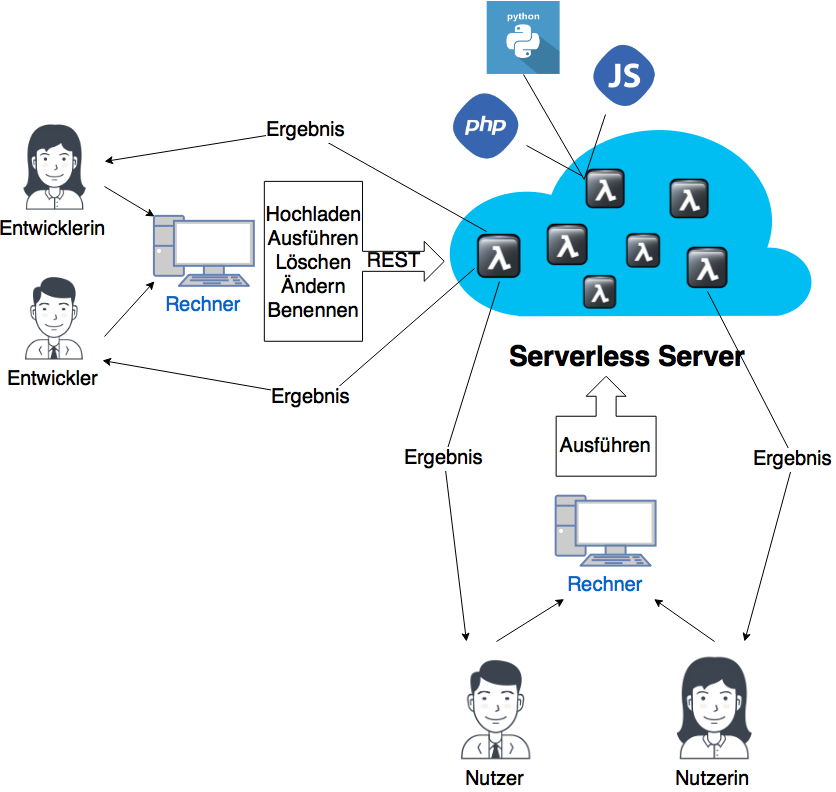
\includegraphics[width=11 cm]{Ubersicht.png}
 \end{center}

Das System lässt sich in drei große Bestandteile aufteilen: \textbf{Gesamtumgebung} (Cloud), \textbf{REST API} und \textbf{\Gls{Docker}-\Gls{Container}} (Lambdas).\\ \\
\textbf{Gesamtumgebung} Die Gesamtumgebung regelt das Zusammenspiel der \Gls{Docker}-\Gls{Container} mit der REST API, den \glspl{Lambda-Funktion} und dem unterliegenden Server.
\\ \\
\textbf{REST API} Die REST API definiert die Kommunikation der \gls{Lambda-Entwickler} und \gls{Lambda-Verwender} mit dem System. Die Hauptfunktionen, die dadurch angesprochen werden sind das Hochladen, Ausführen, Löschen und Ändern der \glspl{Lambda-Funktion}. Die genaue Schnittstelle findet sich unter dem Kapitel zur Benutzerschnittstelle.
\\ \\
\textbf{\Gls{Docker}-\Gls{Container}} Die \Gls{Docker}-\Gls{Container} enthalten die Umgebung für die hochgeladenen \glspl{Lambda-Funktion}. Durch diese wird die Kapselung der \glspl{Lambda-Funktion} geschaffen.
\\
\subsection{Hochladen}
\hspace{1cm}
\begin{center}
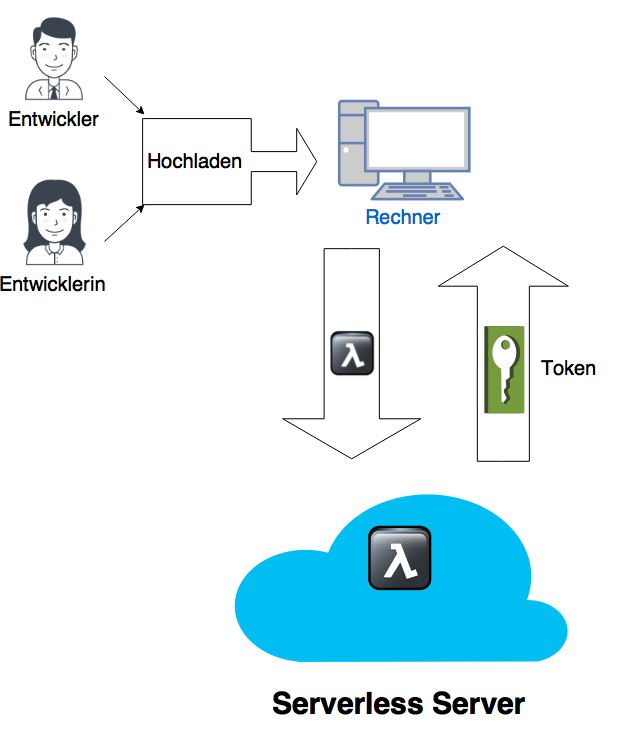
\includegraphics[width=13 cm]{Hochladen.png}
\end{center}

\pagebreak

\subsection{Ausführen}
\hspace{1cm}
\begin{center}
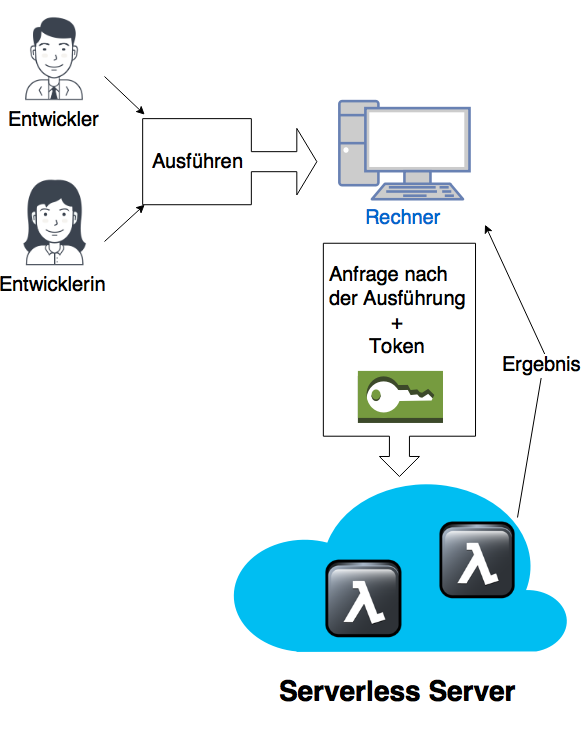
\includegraphics[width=13 cm]{Ausfuhren.png}
\end{center}

\pagebreak

\subsection{Löschen}
\hspace{1cm}
\begin{center}
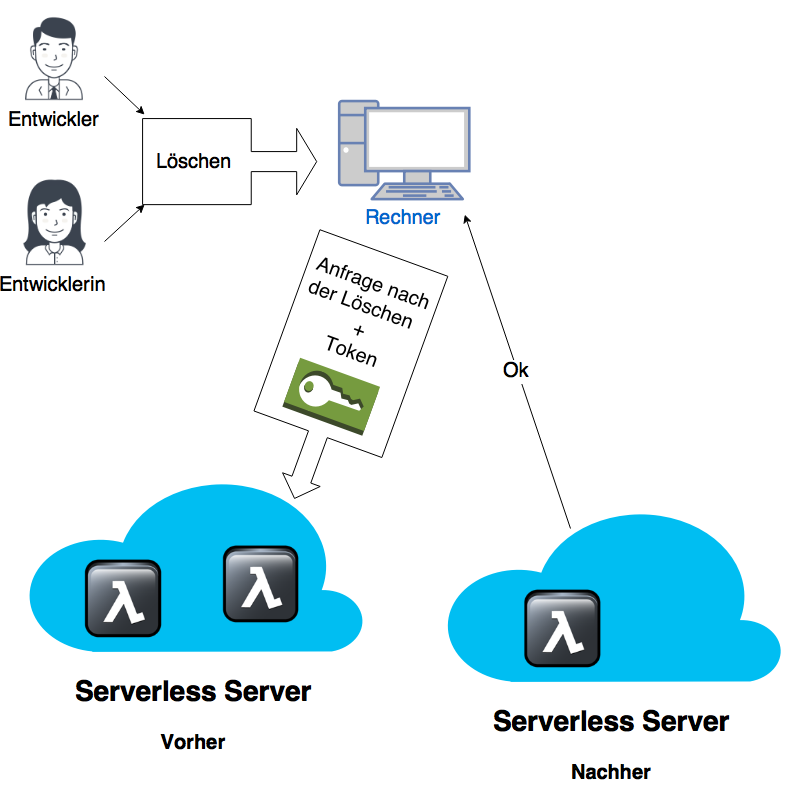
\includegraphics[width=16 cm]{Loschen.png}
\end{center}

\pagebreak

\subsection{Ändern}
\hspace{1cm}
\begin{center}
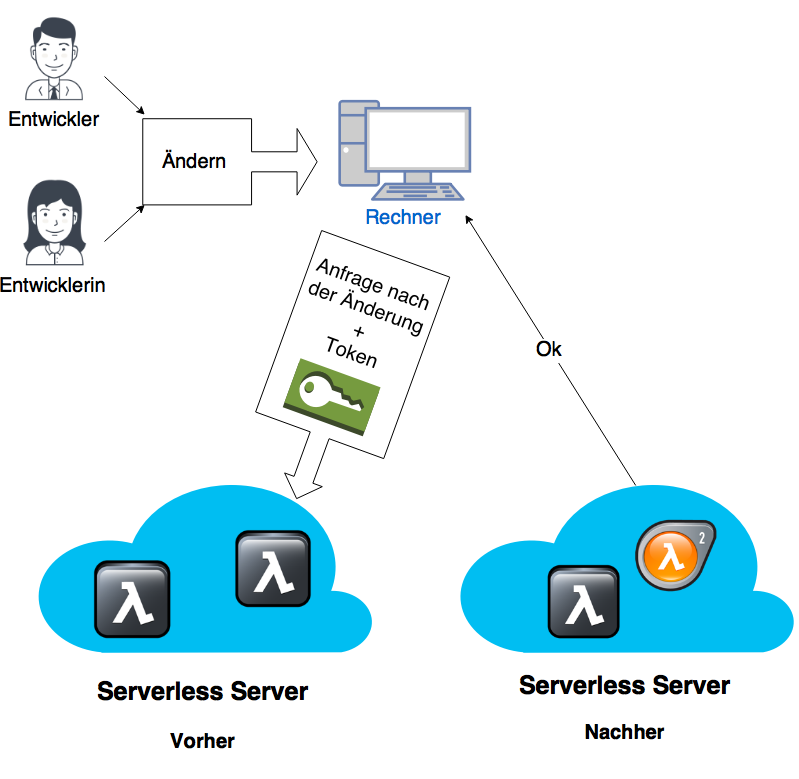
\includegraphics[width=16 cm]{Andern.png} 
\end{center}

\pagebreak

\section{Anwendungsfall: Schokoladenfabrik}
Es gibt eine intelligente Fabrik, die Schokoladenerzeugnisse produziert. Alle ihre Abteilungen sind mit Hilfe vom \gls{Serverless} Server miteinander verbunden. Jede Abteilung schickt Daten an die \glspl{Lambda-Funktion}, die sich auf dem Serverless Server befinden. Dort werden die Daten verarbeitet und anschließend die Ergebnisse zurück an die aufrufende oder andere Abteilungen geschickt. 

\section{Detailszenario: Marketing}
Die Marketingabteilung schickt Verkaufsdaten an eine \gls{Lambda-Funktion} auf dem \gls{Serverless} Server. Diese \gls{Lambda-Funktion} analysiert die Daten und berechnet, welche Schokoladensorten am besten verkauft werden und schickt die Namen der erfolgreichsten Sorten an die Produktionsabteilung. Die Marketingabteilung wird über das Ende des Vorgangs benachrichtigt.
\\
\begin{center}
\includegraphics[width=\linewidth,height=220px ]{marketing.png}
\end{center} 
Im Folgenden werden die Aufgaben der Bestandteile erklärt:
\\ \\
\textbf{Gesamtumgebung} Authentifiziert die Marketing-Abteilung, verarbeitet über REST API gesendete Daten der Marketingabteilung und holt sich aus bestimmten angegebenen Quellen benötigte Ressourcen. Danach startet sie die zugehörige \gls{Lambda-Funktion} in einem \Gls{Docker}-\Gls{Container} mit der verarbeiteten Konfiguration, wartet auf die Beendigung und schickt über die REST API die Fehlermeldung oder das Ergebnis.
\\ \\
\textbf{REST API} Nimmt die Konfiguration für die Ausführung und den Authentifizierungstoken der Marketingabteilung entgegen und schickt ihr nach der Ausführung eine Rückmeldung.
\\ \\
\textbf{\Gls{Docker}-\Gls{Container}} Im \Gls{Container} wird die \gls{Lambda-Funktion}, die die Verkaufsdaten analysiert und die meistverkauften Namen an die Schokoproduktion schickt, ausgeführt.
\\

\pagebreak
\section{Detailszenario: Maschinenwartung}
Wenn eine Maschine defekt ist, wird eine Nachricht an eine \gls{Lambda-Funktion} auf dem \gls{Serverless} Server geschickt. Diese verarbeitet die Nachricht und bestellt z.B die Ersatzteile für die Maschine nach und benachrichtigt Menschen für die Reperatur.
Die Maschine wird  über das Ende des Vorgangs benachrichtigt.
\\
\begin{center}
\includegraphics[width=0.9\linewidth,height=240px]{maschine.png} 
\end{center}

Aufgaben analog zum Detailszenario: Marketing.

\chapter{Benutzerschnittstelle}

\section{Einleitung}
Die Benutzer können die REST \Gls{API} zur Interaktion mit dem System verwenden. Im Folgenden wird zunächst eine Beschreibung der REST \Gls{API} gegeben, die JSON Schnittstelle beschrieben und danach auf ein Beispiel eingegangen, welches das System mithilfe des Programms cURL benutzt.
Die Schnittstellen beschreiben dabei nur die Grundfunktionen aus dem Kapitel über Funktionale Anforderungen.

\section{REST \Gls{API}}
Die \Gls{REST} \Gls{API} unterstützt die neun Befehle GET, POST, PUT, PATCH, DELETE, HEAD, OPTIONS, CONNECT und TRACE. Die folgenden Befehle werden zum Datenaustausch mit dem System verwendet.
\subsection{GET}
Mit GET ist es möglich, Daten von einem \Gls{Server} zu empfangen. Damit kann der \Gls{Lambda-Verwender} beispielsweise die Ergebnisse der Ausführung einer \Gls{Lambda-Funktion} vom Server abrufen.
\subsection{DELETE}
Der Befehl DELETE ermöglicht es, Daten vom Server zu löschen. \Gls{Lambda-Entwickler} können so nicht mehr benötigte oder fehlerhafte \Glspl{Lambda-Funktion} vom Server entfernen.
\subsection{POST}
POST können \Gls{Lambda-Entwickler} verwenden, um dem System neue \Glspl{Lambda-Funktion} hinzuzufügen. Außerdem werden über diesen Befehl die benötigten Daten zur Ausführung einer \Gls{Lambda-Funktion} auf den Server hochgeladen.
\subsection{PUT}
Mit PUT ist es möglich Daten auf dem Server anzupassen. So kann ein \Gls{Lambda-Entwickler} eine neuere Version einer \gls{Lambda-Funktion} auf den Server laden und ausführen. 

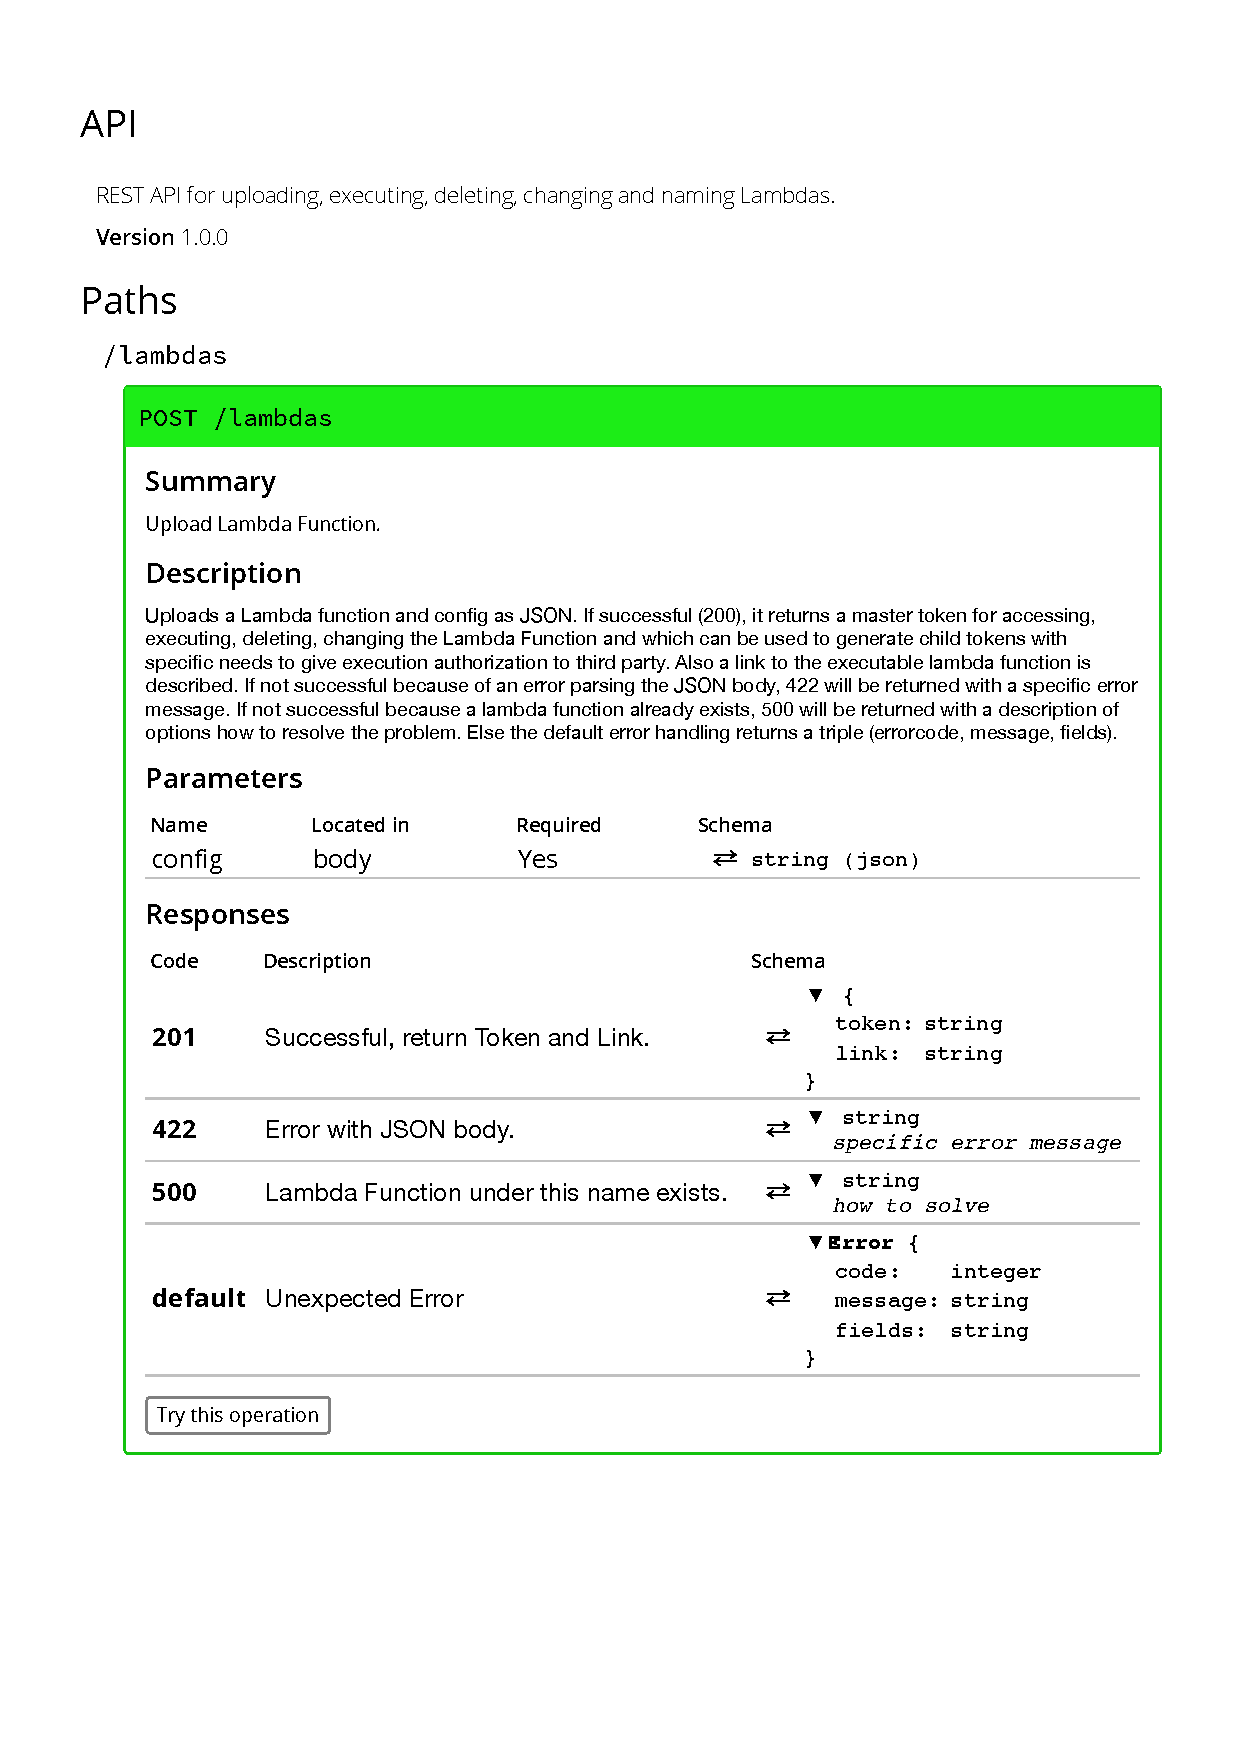
\includepdf[pages={-}]{api.pdf}


\section{Kurzüberblick: JSON Schnittstelle}
Ein Kurzüberblick über die JSON Parameter wird hier gegeben. Eine längere Liste mit ausführlichen Eigenschaften wird im Entwurfsdokument des Systems zu finden sein.

\subsection{Hochladen/Anpassen von Lambda-Funktionen}
Der Absatz beschreibt das Format des Parameters "config" \ beim Hochladen der \gls{Lambda-Funktion}.
\begin{lstlisting}
{
	"name":"<Name_of_Lambda>", #required, id, e.g. lel
	"runtimeAttributes":{
			"language":"<Language_of_Lambda>", #required, programming language, e.g. python3
			"libraries":["library0", "library1"], #required if lamda uses libraries, libraries, e.g. lxml
			"code":"<Code>" #required, json escaped code, e.g. print("Hello world")
	}
}	
\end{lstlisting}
Beim Anpassen der \glspl{Lambda-Funktion} gelten dieselben Regeln wie beim Hochladen. 
Zu beachten ist dabei allerdings, dass ausschließlich die zu ändernden Parameter angegeben werden und andere nicht im Format auftauchen. Leer angegebene Parameter werden auch so interpretiert und der vorherige Stand mit einer leeren Version überschrieben.

\subsection{Ausführung von \glspl{Lambda-Funktion}}
Der Absatz beschreibt das Format des Parameters "config" \ beim Ausführen der \gls{Lambda-Funktion}. Diese darf leer bleiben, sofern keine Parameter benötigt werden. Eine leere Konfiguration sorgt für die einfache Ausführung der  \gls{Lambda-Funktion} ohne Parameter.
\begin{lstlisting}
{
	"times": <number_of_times_running> #not required, number of times running the lambda function (0,maxtimes],
	"parameters_input":[<input0>,<input1>] #required if the lambda function needs arguments to run, e.g. "yolo", "swag", 3 
}
\end{lstlisting}

\newpage

\section{Beispiel: REST \Gls{API} mit cURL}
cURL ist ein Kommandozeilen-Programm zum Übertragen von Dateien in Rechnernetzen.
\begin{lstlisting}
curl
\end{lstlisting}
\subsection{Lambdas hochladen}
\subparagraph{Beispiel: Hochladen als Plaintext}
\begin{lstlisting}
curl -X POST -d '{"name": "lel", "runtimeAttributes":{"language":"python3","code":"print(\"Hello world\")"}}' http://server.less/lambdas
\end{lstlisting}
\begin{lstlisting}
HTTP/1.1 201 Created
Token: eyJhbGciOiJIUzI1NiIsInR5cCI6IkpXVCJ9.eyJzdWIiOiIxMjM0NTY3ODkwIiw
ibmFtZSI6IkpvaG4gRG9lIiwiYWRtaW4iOnRydWV9.TJVA95OrM7E2cBab30RMH
rHDcEfxjoYZgeFONFh7HgQ
Location: /lambdas/lel
\end{lstlisting}
\subsection{Lambdas verändern}
\subparagraph{Beispiel: Verändern als Plaintext}
\begin{lstlisting}
curl -X PUT -d '{"code":"print(\"Bye world\")"}' -H 'token: eyJhbGciOiJIUzI1NiIsInR5cC
I6IkpXVCJ9.eyJzdWIiOiIxMjM0NTY3ODkwIiwibm
FtZSI6IkpvaG4gRG9lIiwiYWRtaW4iOnRydWV9.T
JVA95OrM7E2cBab30RMHrHDcEfxjoYZgeFONFh7HgQ' http://server.less/lambdas/lel
\end{lstlisting}
\begin{lstlisting}
HTTP/1.1 200 OK
\end{lstlisting}
\subsection{Lambdas anzeigen}
\subparagraph{Beispiel: einfache Anzeige}
\begin{lstlisting}
curl -H 'token: eyJhbGciOiJIUzI1NiIsInR5cC
I6IkpXVCJ9.eyJzdWIiOiIxMjM0NTY3ODkwIiwibmFtZSI6IkpvaG4gRG9lIiwiYWR
taW4iOnRydWV9.TJVA95OrM7E2cBab30RMHrHDcEfxjoYZgeFONFh7HgQ' http://server.less/lambdas/lel
\end{lstlisting}
\begin{lstlisting}
HTTP/1.1 200 OK
{"name": "lel",
"runtimeAttributes":{
	"language":"python2",
	"code":"print(\"Bye world\")"
}
}
\end{lstlisting}
\pagebreak
\subsection{Lambdas löschen}
\subparagraph{Beispiel: Löschen}
\begin{lstlisting}
curl -X DELETE -H 'token: eyJhbGciOiJIUzI1NiIsInR5cC
I6IkpXVCJ9.eyJzdWIiOiIxMjM0NTY3ODkwIiwibmFtZSI6IkpvaG4gRG9lIiwiYWR
taW4iOnRydWV9.TJVA95OrM7E2cBab30RMHrHDcEfxjoYZgeFONFh7HgQ'
http://server.less/lambdas/lel
\end{lstlisting}
\begin{lstlisting}
HTTP/1.1 204 No content.
\end{lstlisting}
\subsection{Lambdas ausführen}
\subparagraph{Beispiel: 2x ausführen}
\begin{lstlisting}
curl -X POST -H 'token: eyJhbGciOiJIUzI1NiIsInR5cC
I6IkpXVCJ9.eyJzdWIiOiIxMjM0NTY3ODkwIiwibmFtZSI6IkpvaG4gRG9lIiwiYWR
taW4iOnRydWV9.TJVA95OrM7E2cBab30RMHrHDcEfxjoYZgeFONFh7HgQ'
-d '{"times":"2"}' http://server.less/lambdas/lel/execute
\end{lstlisting}
\begin{lstlisting}
HTTP/1.1 200
Bye world
Bye world
\end{lstlisting}
\subsection{Tokens generieren}
\subparagraph{Beispiel: \glspl{Token} generieren}
\begin{lstlisting}
curl -X GET 
token: eyJhbGciOiJIUzI1
NiIsInR5cCI6IkpXVCJ9.eyJzdWIiOiIxMjM0NTY3ODkwIiwibmFtZSI6IkpvaG4g
RG9lIiwiYWRtaW4iOnRydWV9.TJVA95OrM7E2cBab30RMHrHDcEfxjoYZgeFONFh7HgQ'
http://server.less/lambdas/lel/token
\end{lstlisting}
\begin{lstlisting}
HTTP/1.1 200 OK eyJhbGciOiJIUzI1NiIsInR5cCI6IkpXVCJ9.eyJzdWIiOiIxMjM0NTY3ODkw
IiwibmFtZSI6IkpvaG4gRG9lIiwiYWRtaW4iOnRydWV9.TJVA95OrM7E2
cBab30RMHrHDcEfxjoYZgeFONFh7HgQ
\end{lstlisting}

\chapter{Qualitätsbestimmungen}

\begin{table}[H]
\centering
\begin{tabular}{|l| l l l l|}
\hline \\
 \textbf{Produktqualität} & \textbf{Sehr gut} & \textbf{Gut} & \textbf{Normal} & \textbf{Nicht relevant} \\\\ \hline \hline \\
 \textbf{Funktionalität} &  &  &  &  \\ \hline \\
 Angemessenheit & & X &  &  \\
 Richtigkeit &  &  &  & X  \\
 Interoperablilität & X &  &  &  \\
 Ordnungsmäßigkeit &  &  &  & X \\
 Sicherheit &  & X &  &  \\ 
 Konformität & X &  &  &  \\ \hline\hline \\
 \textbf{Zuverlässigkeit} &  &  &  &  \\ \hline \\
 Fehlertoleranz &  & X &  &  \\
 Verfügbarkeit &  & X &  &  \\ \hline\hline \\
 \textbf{Benutzbarkeit} &  &  &  &  \\ \hline \\
 Verständlichkeit &  &  & X &  \\
 Erlernbarkeit &  & X &  &  \\
 Bedienbarkeit &  & X &  &  \\ \hline\hline \\
 \textbf{Effizienz} &  &  &  &  \\ \hline \\
 Zeitverhalten &  & X  &  &  \\
 Verbrauchsverhalten &  & X &  &  \\ \hline\hline \\
 \textbf{Übertragbarkeit} &  &  &  &  \\ \hline \\
 Anpassbarkeit & X &  &  &  \\
 Installierbarkeit & X &  &  &  \\
 Austauschbarkeit &  & X &  & \\ \hline\hline
\end{tabular}
\caption{Übersicht der Qualitätsbestimmungskriterien}
\end{table}

\section{Funktionalität}

\subsection{Angemessenheit: gut}

\textbf{Definition} \\
Eignung von \glspl{Lambda-Funktion} für spezifizierte Aufgaben, zum Beispiel aufgabenorientierte Zusammensetzung von \glspl{Lambda-Funktion} aus Teilfunktionen.  \\ \\
\textbf{Begründung} \\
Da das Ziel ist, einen möglichst allgemein benutzbaren Server zum Hochladen und Ausführen von \glspl{Lambda-Funktion} zu entwickeln, müssen die \glspl{Lambda-Funktion} des Servers für verschieden spezifizierte Aufgaben genügen.

\subsection{Richtigkeit: nicht relevant}

\textbf{Definition} \\
Liefern der richtigen oder vereinbarten Ergebnisse oder Wirkungen, zum Beispiel die benötigte Genauigkeit von berechneten Werten. \\ \\
\textbf{Begründung} \\
Da die auf dem Server ausgeführten \glspl{Lambda-Funktion} von externen \gls{Lambda-Entwickler}n stammen, sind diese für die Richtigkeit der zurückgegebenen Werte verantwortlich.

\subsection{Interoperabilität: sehr gut}

\textbf{Definition} \\
Fähigkeit, mit vorgegebenen Systemen zusammenzuwirken. \\ \\
\textbf{Begründung} \\
Da das Produkt vor allem auf die Verwendung als externer Rechner abzielt, muss vor allem die Schnittstelle, aber auch das Gesamtprodukt sehr gute Interoperabilität besitzen.

\subsection{Ordnungsmäßigkeit: nicht relevant}

\textbf{Definition} \\
Merkmale von Software, die bewirken, dass die Software anwendungsspezifische Normen oder Vereinbarungen oder gesetzliche Bestimmungen und ähnliche Vorschriften erfüllt. \\ \\
\textbf{Begründung} \\
Da die auf dem Server ausgeführten \glspl{Lambda-Funktion} von externen \gls{Lambda-Entwickler}n stammen, sind diese für die Ordnungsmäßigkeit verantwortlich.

\subsection{Sicherheit: gut}

\textbf{Definition} \\
Fähigkeit, unberechtigten Zugriff, sowohl versehentlich als auch vorsätzlich, auf Programme und Daten zu verhindern.\\ \\
\textbf{Begründung}
Da in dem Produkt mehrere \glspl{Lambda-Funktion} verschiedener \gls{Lambda-Entwickler} nebeneinander auf einem Server liegen, muss sichergestellt werden, dass weder Programm noch Mensch auf nicht auf \glspl{Lambda-Funktion} Zugriff haben, wenn sie nicht berechtigt sind.

\subsection{Konformität: sehr gut}

\textbf{Definition} \\
Fähigkeit des Softwareprodukts, Standards, Konventionen oder gesetzliche Bestimmungen und ähnliche Vorschriften bezogen auf die Funktionalität einzuhalten. \\ \\
\textbf{Begründung}\\
Da die Interoperabilität schwer ohne Konformität zu erreichen ist, ist die Einhaltung dieses Kriteriums wichtig.
\\
\section{Zuverlässigkeit}

\subsection{Fehlertoleranz: gut}

\textbf{Definition} \\
Fähigkeit, ein spezifiziertes Leistungsniveau bei Software-Fehlern oder Nicht-Einhaltung ihrer spezifizierten Schnittstelle zu bewahren.
Konformität: Grad, in dem die Software Normen oder Vereinbarungen zur Zuverlässigkeit erfüllt. \\ \\
\textbf{Begründung} \\
Da verschiedene \glspl{Lambda-Funktion} von verschiedenen \gls{Lambda-Entwickler}n gleichzeitig auf dem Server liegen, muss eine gewisse Fehlertoleranz geschaffen werden, da sonst z.B. bei einem Absturz viele \gls{Lambda-Verwender} betroffen wären.

\subsection{Verfügbarkeit: Gut}

\textbf{Definition} \\
Wahrscheinlichkeitsmaß, dass das System bestimmte Anforderungen zu bzw. innerhalb eines vereinbarten Zeitrahmens erfüllt.\\ \\
\textbf{Begründung} \\
Die Verfügbarkeit ist ein wichtiges Kriterium, dass mit der Begründung zur Fehlertoleranz einhergeht.
\\
\section{Benutzbarkeit}

\subsection{Verständlichkeit: normal}

\textbf{Definition} Aufwand für den Benutzer, das Konzept und die Anwendung zu verstehen. \\ \\
\textbf{Begründung} \\
Da das Hauptklientel des Produktes \gls{Lambda-Entwickler} sind, welche ein Verständnis für die Produktteile haben, ist der Aufwand normal hoch, um sich mit dem Produkt vertraut zu machen.

\subsection{Erlernbarkeit: gut}

\textbf{Definition} Aufwand für den Benutzer, die Anwendung zu erlernen. \\ \\
\textbf{Begründung} \\
Da das Hauptklientel des Produktes \gls{Lambda-Entwickler} sind, welche ein Verständnis für die geläufigen Schnittstellen haben, ist der Aufwand gering, um sich mit den Schnittstellen vertraut zu machen.

\subsection{Bedienbarkeit: gut}

\textbf{Definition} \\
Aufwand für den Benutzer, die Anwendung zu bedienen. \\ \\
\textbf{Begründung} \\
Da \gls{REST} sehr geläufig und einfach ist und es viele Anleitungen und Bedienungsmöglichkeiten dazu existieren, ist der Aufwand sehr gering.
\\
\section{Effizienz}

\subsection{Zeitverhalten: gut}

\textbf{Definition} \\
Antwort- und Verarbeitungszeiten sowie Durchsatz bei der Funktionsausführung. \\ \\
\textbf{Begründung} \\
Da die Antwort- und Verarbeitungszeiten von der jeweiligen \gls{Lambda-Funktion} abhängen ist diese von den \gls{Lambda-Entwickler}n und \gls{Lambda-Verwender}n abhängig. Das Übertragen und die Vorbereitungen für die Ausführung sollten allerdings minimal gehalten werden.

\subsection{Verbrauchsverhalten: gut}

\textbf{Definition} \\
Anzahl und Dauer der benötigten Betriebsmittel bei der Erfüllung der \glspl{Lambda-Funktion}. \\ \\
\textbf{Begründung} \\
Da das Verbrauchsverhalten ebenso mehrheitlich von den jeweiligen \gls{Lambda-Funktion} abhängen, ist nur die Minimierung der Betriebsmittelbeschaffung zu beachten.

\section{Übertragbarkeit}

\subsection{Anpassbarkeit: sehr gut}

\textbf{Definition} \\
Fähigkeit der Software, diese an verschiedene Umgebungen anzupassen. \\ \\
\textbf{Begründung} \\
Da das System auf verschiedenen Umgebungen laufen muss, ist die Anpassbarkeit ein wichtiges Kriterium.

\subsection{Installierbarkeit: sehr gut}

\textbf{Definition} \\
Aufwand, der zum Installieren der Software in einer festgelegten Umgebung notwendig ist. \\ \\
\textbf{Begründung} \\
Da das System auf verschiedenen Umgebungen laufen muss, ist die Minimierung des Installationsaufwands ein wichtiges Kriterium.

\subsection{Austauschbarkeit: gut}

\textbf{Definition} \\
Möglichkeit, diese Software anstelle einer spezifizierten anderen in der Umgebung jener Software zu verwenden, sowie der dafür notwendige Aufwand. \\ \\
\textbf{Begründung} \\
Da das System zur Ausführung von \glspl{Lambda-Funktion} durch andere Systeme ersetzbar sein sollte, muss die Austauschbarkeit vereinfacht werden.


\chapter{Testfälle und Szenarien}
\section{Testfälle}
\subsection{Funktionen}
\begin{longtable}{lp{10cm}p{3cm}}
\hline \\
\textbf{Nr.} & \textbf{Beschreibung} & \textbf{Kriterium} \\ \hline\hline \\ 
/T010/ & \Gls{Lambda-Entwickler} lädt eine \gls{Lambda-Funktion} hoch und bekommt ein Zugriffs-\gls{Token} zurück. & /F010/, /F011/   \\ \hline \\
/T020/ & \Gls{Lambda-Entwickler} führt die \gls{Lambda-Funktion} mit seinem Zugriffs-\gls{Token} aus. & /F020/\\ \hline \\
/T021/ & \Gls{Lambda-Entwickler} stellt die Ausführungsumgebung für die \gls{Lambda-Funktion} bereit. & /F021/\\ \hline \\
/T030/ & \Gls{Lambda-Entwickler} gibt \glspl{Token} für \Gls{Lambda-Verwender} aus. & /F110/\\ \hline \\
/T040/ & \Gls{Lambda-Entwickler} authentifiziert sich. & /F100/\\ \hline \\
/T050/ & \Gls{Lambda-Entwickler} löscht seine \gls{Lambda-Funktion}. & /F030/, /F031/\\ \hline \\
/T051/ & \Gls{Lambda-Entwickler} ändert seine \gls{Lambda-Funktion}. & /F040/\\ \hline \\
/T052/ & \Gls{Lambda-Entwickler} benennt seine \gls{Lambda-Funktion}. & /F050/\\ \hline \\
/T053/ & \Gls{Lambda-Entwickler} konfiguriert seine \gls{Lambda-Funktion}. & /F050/\\ \hline \\
/T054/ & \Gls{Lambda-Entwickler} bindet Daten für seine \gls{Lambda-Funktion} ein. & /F050/\\ \hline \\
/T060/ & \Gls{Lambda-Verwender} führt eine \gls{Lambda-Funktion} mit einem \gls{Token} aus. & /F020/\\ \hline \\
/T061/ & \Gls{Lambda-Verwender} gibt an, wie oft die \gls{Lambda-Funktion} ausgeführt werden muss. & \\ \hline \\
/T070/ & Gleichzeitiger Zugriff auf eine hochgeladene \gls{Lambda-Funktion} von mehreren Rechnern aus. & \\ \hline \\
/T080/ & Terminierung einer \gls{Lambda-Funktion}. & /F080/\\ \hline \\
/T090/ & Eine Lambda-Funktion, die länger läuft als vom Server vorgegeben, wird terminiert. & /NF030/\\ \hline 
\hline
\\\\
\end{longtable}

\subsection{Testfalle für unzulässige Aktionen}
\begin{longtable}{lp{10cm}p{3cm}}
\hline \\
\textbf{Nr.} & \textbf{Beschreibung} & \textbf{Kriterium} \\ \hline\hline \\
/UT010/ & \Gls{Lambda-Verwender} ruft eine nicht-existierende \gls{Lambda-Funktion} auf. & \\ \hline \\
/UT020/ & \Gls{Lambda-Verwender} ruft eine \gls{Lambda-Funktion} mit einem falschen \gls{Token} auf. & /F020/\\ \hline \\
/UT030/ & \Gls{Lambda-Entwickler} gibt ein zu langes Zeitintervall für eine Funktionsausführung an. & bezieht sich auf /WT010/\\  \hline 
\hline
\\\\
\end{longtable}

\subsection{Testfalle für Wünschkriterien}
\begin{longtable}{lp{10cm}p{3cm}}
\hline \\
\textbf{Nr.} & \textbf{Beschreibung} & \textbf{Kriterium} \\ \hline\hline \\ 
/WT010/ & \Gls{Lambda-Entwickler} gibt eine Höchst-Laufzeit für seine \gls{Lambda-Funktion} an. & /F140/ \\ \hline \\
/WT020/ & Ein Zähler zu den \glspl{Token} wird erstellt. & /F150/\\ \hline \\
/WT021/ & \Gls{Lambda-Entwickler} ließt den \gls{Token}-Zähler aus. & /F160/\\ \hline \\
/WT030/ & \Gls{Lambda-Entwickler} spezifiziert Firewalleinstellungen für seine \gls{Lambda-Funktion}. & /F190/\\ \hline \\
/WT040/ & \Gls{Lambda-Entwickler} gibt ein \Gls{Repository} an. & /F170/\\ \hline \\
/WT050/ & \Gls{Lambda-Entwickler} lädt eine \gls{Lambda-Funktion} von dem angegebenen \Gls{Repository} auf den \Gls{Server}. & /F170/\\ \hline \\
/WT060/ & \Gls{Lambda-Verwender} oder \Gls{Lambda-Entwickler} spezifiziert die Zeit für die Bereitstellung des Ergebnisses der \gls{Lambda-Funktion}. & /F200/\\ \hline \\
/WT070/ & \Gls{Lambda-Entwickler} kauft die \glspl{Token} für seine \gls{Lambda-Funktion}. &/F210/\\ \hline \\
/WT080/ & \Gls{Lambda-Entwickler} ersetzt die aktuelle \gls{Lambda-Funktion} durch ihre frühere Version. &/F180/\\ \hline \\
/WT090/ & Serverbetreiber greift auf die Statistiken für die \Glspl{Lambda-Funktion} zu.&/F220/\\ \hline 
\hline
\\
\end{longtable}
\newpage
\section{Testszenarien}
\subsection{\gls{Lambda-Entwickler} lädt seine \gls{Lambda-Funktion} hoch}
Ein \Gls{Lambda-Entwickler} lädt eine \gls{Lambda-Funktion} mit ihrem Namen, Angabe der Sprache, ggf. Adresse von zusätzlichen Dateien und dem Code selbst mit dem Befehl POST hoch. Falls die Eingabe korrekt ist, bekommt er eine Bestätigung, den Speicherort der erstellten \gls{Lambda-Funktion} und den Zugriffs-\gls{Token} als Antwort, sonst bekommt er eine Fehlermeldung mit dem Fehlercode zurück.\\\\
\textbf{Wunschfunktion 1}: der \Gls{Lambda-Entwickler} gibt anstatt von Code die Adresse von eines \Gls{Repository} an, in welchem die \gls{Lambda-Funktion} gespeichert ist.\\\\
\textbf{Wunschfunktion 2}: der \Gls{Lambda-Entwickler} kann zusätzlich eine maximale Laufzeit und Firewall-Einstellungen für seine \gls{Lambda-Funktion} angeben.\\

\begin{enumerate}
\item /T010/ \Gls{Lambda-Entwickler} lädt eine \gls{Lambda-Funktion} hoch und bekommt ein Zugriffs-\gls{Token} zurück.
\item /T021/ \Gls{Lambda-Entwickler} stellt die Ausführungsumgebung für die \gls{Lambda-Funktion} bereit.
\item /T040/ \Gls{Lambda-Entwickler} authentifiziert sich.
\item /T052/ \Gls{Lambda-Entwickler} benennt seine \gls{Lambda-Funktion}. 
\item /T053/ \Gls{Lambda-Entwickler} konfiguriert seine \gls{Lambda-Funktion}. 
\item /T054/ \Gls{Lambda-Entwickler} bindet Daten für seine \gls{Lambda-Funktion} ein.
\item /WT040/ \Gls{Lambda-Entwickler} gibt ein \Gls{Repository} an.
\item /WT010/ \Gls{Lambda-Entwickler} gibt eine Laufzeit für seine \gls{Lambda-Funktion} an.
\item /WT030/ \Gls{Lambda-Entwickler} spezifiziert Firewalleinstellungen für seine \gls{Lambda-Funktion}.
\\
\end{enumerate} 

\subsection{\gls{Lambda-Entwickler} ändert seine Funktion}
Ein \Gls{Lambda-Entwickler} lädt eine veränderte \gls{Lambda-Funktion} mit ihrem Namen, dem Zugriffs-\gls{Token} und dem Code selbst mit dem Befehl PUT hoch. Falls die Eingabe korrekt ist, bekommt er eine Bestätigung als Antwort, sonst bekommt er eine Fehlermeldung mit dem Fehlercode zurück.\\\\
\textbf{Wunschfunktion 1}: der \Gls{Lambda-Entwickler} gibt anstatt von dem geänderten Code die Adresse eines \Gls{Repository} an, in welchem die veränderte \gls{Lambda-Funktion} gespeichert ist.\\
\begin{enumerate}
\item /T051/ \Gls{Lambda-Entwickler} ändert seine \gls{Lambda-Funktion}.
\item /T040/ \Gls{Lambda-Entwickler} authentifiziert sich (mittels eines Zugriffs-\gls{Token}).
\item /WT050/ \Gls{Lambda-Entwickler} lädt eine veränderte \gls{Lambda-Funktion} von dem angegebenen \Gls{Repository} auf den Server.
\item /WT080/ \Gls{Lambda-Entwickler} ersetzt die aktuelle \gls{Lambda-Funktion} durch ihre frühere Version.
\\
\end{enumerate} 
\subsection{\gls{Lambda-Entwickler} ruft die Einstellungen seiner Funktion auf}
Ein \Gls{Lambda-Entwickler} gibt den Befehl GET, den Namen der \gls{Lambda-Funktion} und den Zugriffs-\gls{Token} ein. Falls die Eingabe korrekt ist, bekommt er eine Bestätigung und die Einstellungen der \gls{Lambda-Funktion} als Antwort. Im anderen Fall bekommt er eine Fehlermeldung mit dem Fehlercode zurück.\\
\subsection{\gls{Lambda-Entwickler} löscht seine Funktion}
Ein \Gls{Lambda-Entwickler} gibt den Befehl DELETE, den Namen der \gls{Lambda-Funktion} und den Zugriffs-\gls{Token} ein. Falls die Eingabe korrekt ist, bekommt er eine Bestätigung, und alle laufende Instanzen der \gls{Lambda-Funktion} werden folgend beendet (nach /F031/). Im anderen Fall bekommt er eine Fehlermeldung mit dem Fehlercode zurück.\\
\begin{enumerate}
\item /T050/ \Gls{Lambda-Entwickler} löscht seine \gls{Lambda-Funktion}.
\item /T040/ \Gls{Lambda-Entwickler} authentifiziert sich (mittels eines Zugriffs-\gls{Token}).
\\
\end{enumerate} 


\subsection{\gls{Lambda-Verwender} ruft eine \gls{Lambda-Funktion} auf}
Ein \Gls{Lambda-Verwender} authentifiziert sich mittels eines \gls{Token}s und gibt den Befehl POST mit der Adresse der zu ausführenden Funktion, den möglichen Parametern und der Anzahl der Ausführungen ein. Die \gls{Lambda-Funktion} wird ausgeführt, falls sie unter gegebener Adresse existiert, und wird eventuell nach einer vom Server oder vom \Gls{Lambda-Verwender} spezifizierten Zeit abgebrochen. Als Antwort bekommt der \Gls{Lambda-Verwender} eine Bestätigung und das Ergebnis der Ausführung(en), oder er bekommt eine Fehlermeldung mit dem Fehlercode zurück.\\\\
\textbf{Wunschfunktion 1}: der \Gls{Lambda-Verwender} kann die Zeit angeben, wann die Ergebnisse der \gls{Lambda-Funktion} bereitgestellt werden.\\

\begin{enumerate}
\item /T060/ \Gls{Lambda-Verwender} führt eine \gls{Lambda-Funktion} mit einem \gls{Token} aus.
\item /T061/ \Gls{Lambda-Verwender} gibt an, wie oft die \gls{Lambda-Funktion} ausgeführt werden muss.
\item /T080/ Terminierung einer \gls{Lambda-Funktion}.
\item /T090/ Eine Lambda-Funktion, die länger läuft als vom Server vorgegeben, wird terminiert.
\item ggf. /T070/ Gleichzeitiger Zugriff auf eine hochgeladene \gls{Lambda-Funktion} von mehreren Rechnern aus.
\item /UT020/ \Gls{Lambda-Verwender} ruft eine nicht-existierende \gls{Lambda-Funktion} auf.
\item /UT030/ \Gls{Lambda-Verwender} ruft eine \gls{Lambda-Funktion} mit einem falschen \gls{Token} aus.
\item /WT060/ \Gls{Lambda-Verwender} spezifiziert die Zeit für die Bereitstellung des Ergebnisses der \gls{Lambda-Funktion}.
\item /WT010/ Abbruch von Lambda-Funktionen.
\\
\end{enumerate} 
\subsection{\gls{Lambda-Entwickler} generiert einen Child-Token für \gls{Lambda-Verwender}}
Ein \Gls{Lambda-Entwickler} gibt seinen Zugriffs-\gls{Token}, die Funktionsparameter und die Adresse der \gls{Lambda-Funktion} mit dem Befehl GET ein. Als Antwort erhält er eine Bestätigung und einen Child-Token für die zukünftigen \Glspl{Lambda-Verwender} oder er bekommt eine Fehlermeldung mit dem Fehlercode zurück.\\\\
\textbf{Wunschfunktion 1}: der \Gls{Lambda-Entwickler} kann zusätzliche \glspl{Token} für seine \gls{Lambda-Funktion} kaufen.\\\\
\textbf{Wunschfunktion 1}: der \Gls{Lambda-Entwickler} kann einen Zähler für seine Child-Tokens erstellen.\\
\begin{enumerate}
\item /T030/ \Gls{Lambda-Entwickler} gibt \glspl{Token} für \Glspl{Lambda-Verwender} aus.
\item /T040/ \Gls{Lambda-Entwickler} authentifiziert sich. 
\item /WT070/ \Gls{Lambda-Entwickler} kauft die \glspl{Token} für seine \gls{Lambda-Funktion}.
\item /WT020/ \Gls{Lambda-Entwickler} erstellt einen Zähler zu den \glspl{Token}.
\\
\end{enumerate} 
\chapter{Entwicklungsumgebung}
\section{Betriebssysteme}
\begin{itemize}
\item Mac OS X
\item Windows
\item Linux
\end{itemize}

\section{Entwicklung}
\begin{itemize}
\item Entwicklungsumgebung \Gls{IntelliJ} für die Java-Entwicklung. 
\item  Entwicklungsumgebung \Gls{Eclipse} für die Java-Entwicklung.
\end{itemize}

\section{Versionsverwaltung}
\begin{itemize}
\item Git
\end{itemize}

\section{Sonstige verwendete Software}
\begin{itemize}
\item LaTeX für die zu erstellenden Dokumente (z. B. Pflichtenheft)
\item\Gls{Docker}
\end{itemize}

\section{Hardware}
\begin{itemize}
\item Standard-PCs
\item Standard-Laptops
\item Server zum Testen der Software
\end{itemize}

\printglossaries
\end{document}